\documentclass[11pt]{article}
\usepackage[textwidth=18.0cm, textheight=23.0cm, top=2.0cm]{geometry}
\usepackage{pst-all}
\usepackage{amssymb}
\usepackage{tikz}
\usepackage{underscore}\begin{document}
\pagestyle{empty}


ClassName: \underline{\textbf{Class_03.2bp-38}}
\par
BinSize: \underline{\textbf{40 × 40}}
\par
ReduceSize: \underline{\textbf{40 × 40}}
\par
TypeNum: \underline{\textbf{78}}
\par
Num: \underline{\textbf{80}}
\par
OutS: \underline{\textbf{33600}}
\par
InS: \underline{\textbf{29756}}
\par
Rate: \underline{\textbf{0.886}}
\par
UB: \underline{\textbf{21}}
\par
LB0: \underline{\textbf{21}}
\par
LB: \underline{\textbf{21}}
\par
LBWithCut: \underline{\textbf{21}}
\par
NodeCut: \underline{\textbf{0}}
\par
ExtendedNodeCnt: \underline{\textbf{1}}
\par
GenNodeCnt: \underline{\textbf{1}}
\par
PrimalNode: \underline{\textbf{0}}
\par
ColumnCount: \underline{\textbf{21}}
\par
TotalCutCount: \underline{\textbf{0}}
\par
RootCutCount: \underline{\textbf{0}}
\par
LPSolverCnt: \underline{\textbf{1}}
\par
PricingSolverCnt: \underline{\textbf{0}}
\par
BranchAndBoundNum: \underline{\textbf{1}}
\par
isOpt: \underline{\textbf{true}}
\par
TimeOnInitSolution: \underline{\textbf{600.000 s}}
\par
TimeOnPrimal: \underline{\textbf{0.000 s}}
\par
TimeOnPricing: \underline{\textbf{0.000 s}}
\par
TimeOnRmp: \underline{\textbf{0.062 s}}
\par
TotalTime: \underline{\textbf{600.328 s}}
\par
\newpage


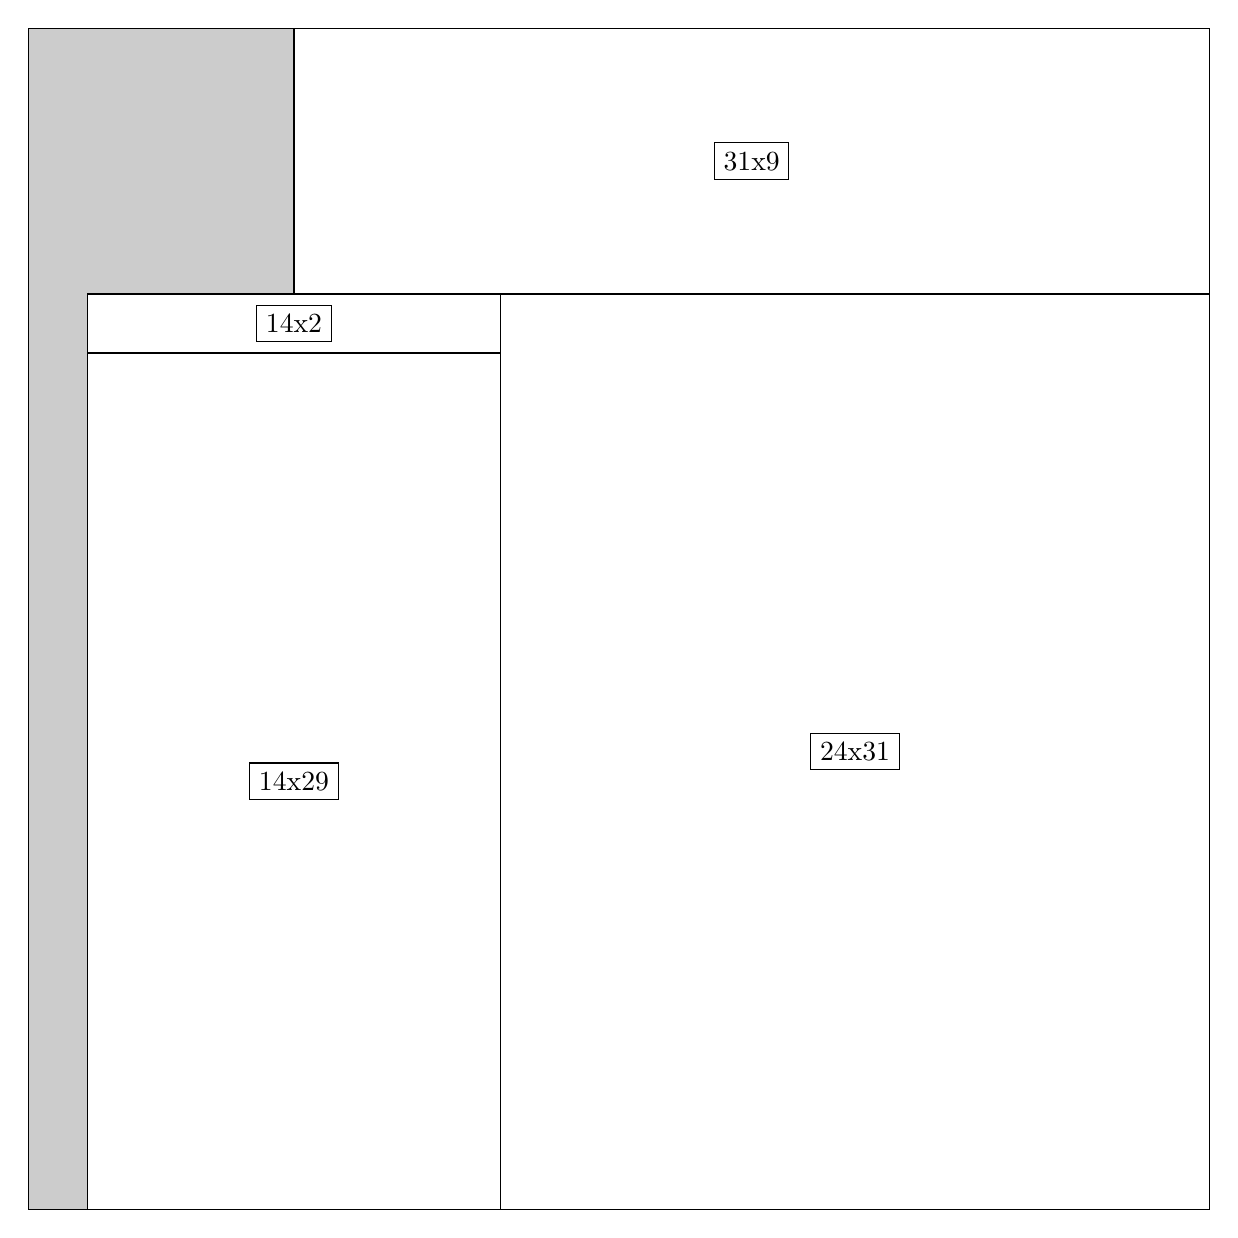
\begin{tikzpicture}[shorten >=1pt,scale=1.0,every node/.style={scale=1.0},->]
\tikzstyle{vertex}=[circle,fill=black!25,minimum size=14pt,inner sep=0pt]
\filldraw[fill=gray!40!white, draw=black] (0,0) rectangle (15.0,15.0);
\foreach \name/\x/\y/\w/\h in {24x31/6.0/0.0/9.0/11.625,14x29/0.75/0.0/5.25/10.875,14x2/0.75/10.875/5.25/0.75,31x9/3.375/11.625/11.625/3.375}
\filldraw[fill=white!40!white, draw=black] (\x,\y) rectangle node[draw] (\name) {\name} ++(\w,\h);
\end{tikzpicture}


w =24 , h =31 , x =16 , y =0 , v =744
\par
w =14 , h =29 , x =2 , y =0 , v =406
\par
w =14 , h =2 , x =2 , y =29 , v =28
\par
w =31 , h =9 , x =9 , y =31 , v =279
\par
\newpage


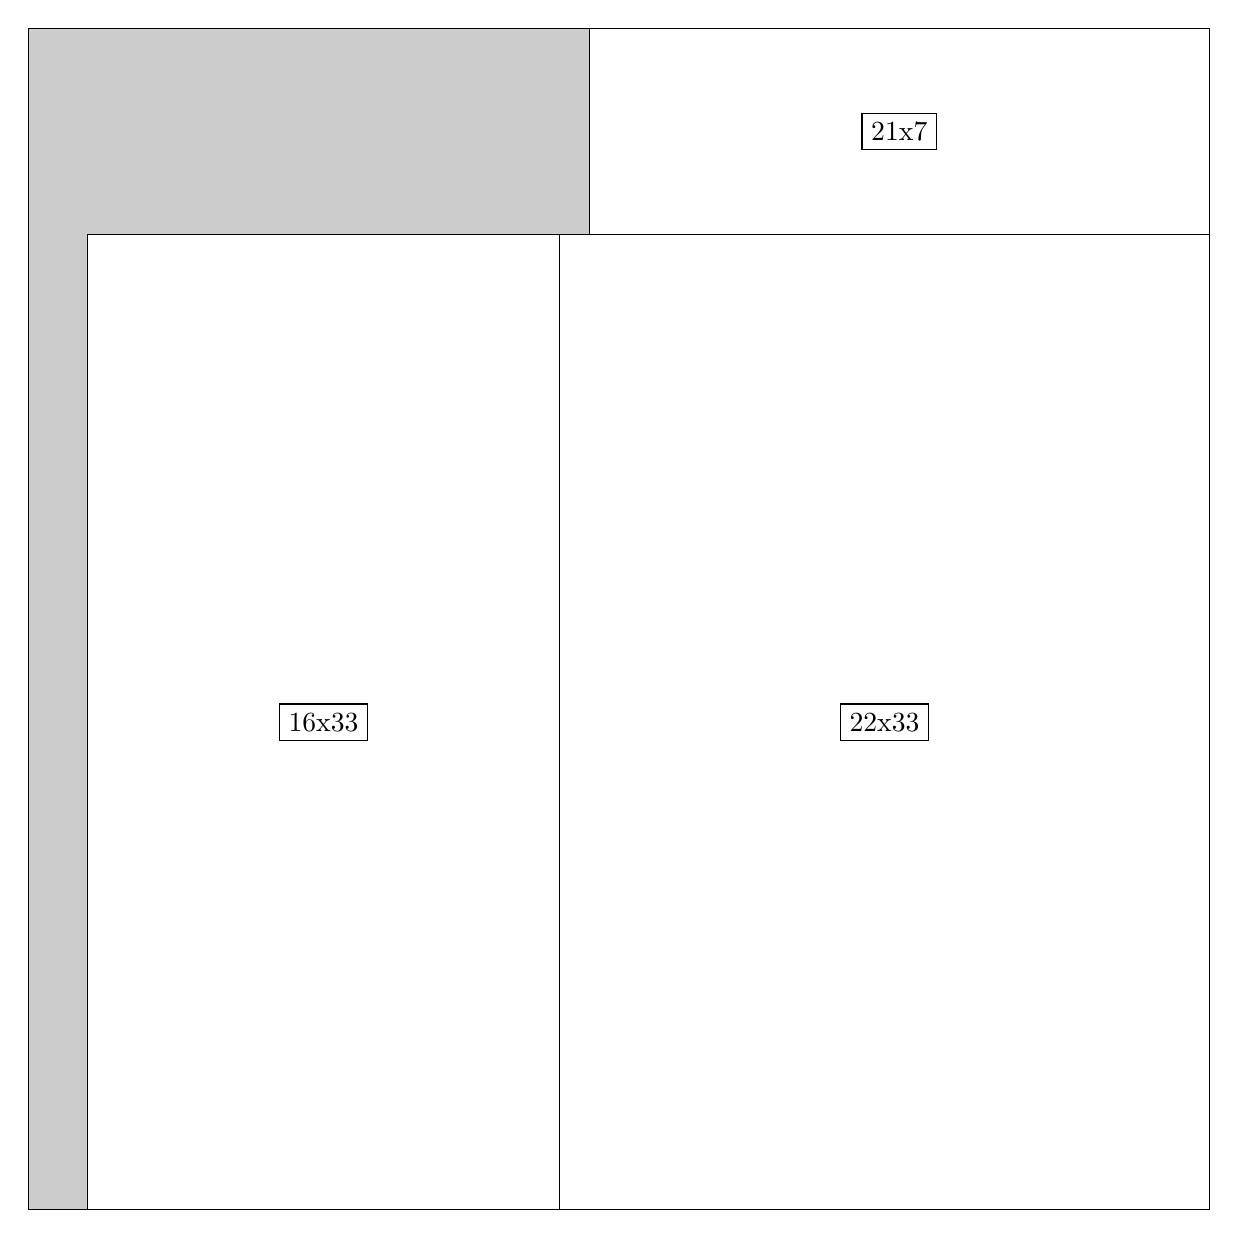
\begin{tikzpicture}[shorten >=1pt,scale=1.0,every node/.style={scale=1.0},->]
\tikzstyle{vertex}=[circle,fill=black!25,minimum size=14pt,inner sep=0pt]
\filldraw[fill=gray!40!white, draw=black] (0,0) rectangle (15.0,15.0);
\foreach \name/\x/\y/\w/\h in {22x33/6.75/0.0/8.25/12.375,16x33/0.75/0.0/6.0/12.375,21x7/7.125/12.375/7.875/2.625}
\filldraw[fill=white!40!white, draw=black] (\x,\y) rectangle node[draw] (\name) {\name} ++(\w,\h);
\end{tikzpicture}


w =22 , h =33 , x =18 , y =0 , v =726
\par
w =16 , h =33 , x =2 , y =0 , v =528
\par
w =21 , h =7 , x =19 , y =33 , v =147
\par
\newpage


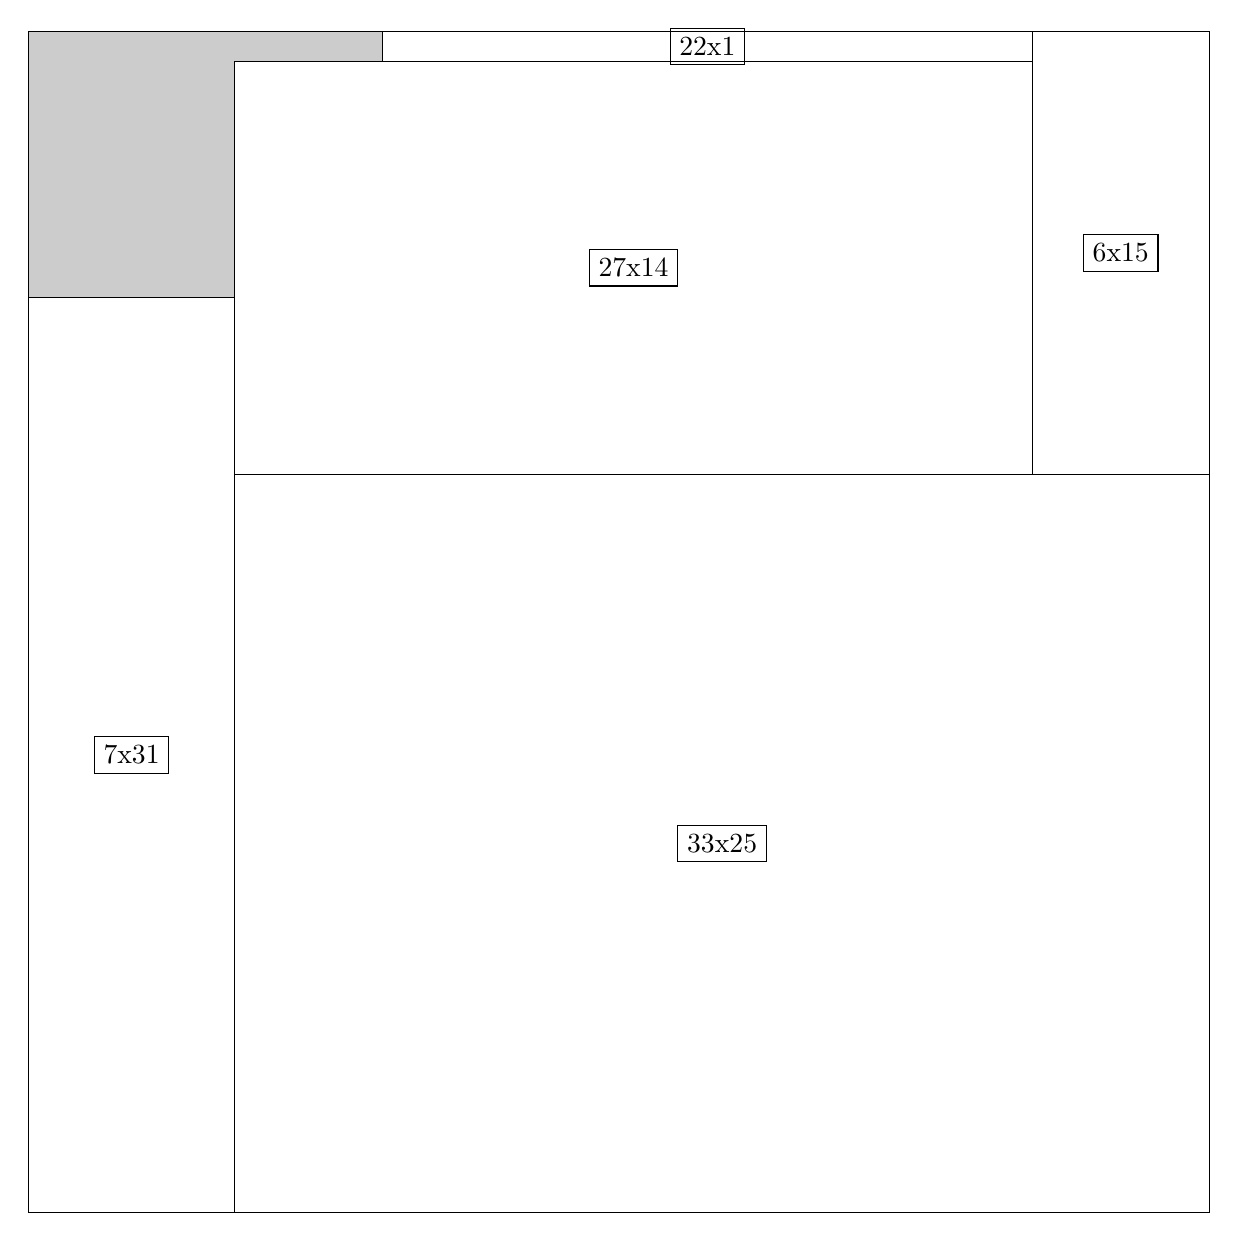
\begin{tikzpicture}[shorten >=1pt,scale=1.0,every node/.style={scale=1.0},->]
\tikzstyle{vertex}=[circle,fill=black!25,minimum size=14pt,inner sep=0pt]
\filldraw[fill=gray!40!white, draw=black] (0,0) rectangle (15.0,15.0);
\foreach \name/\x/\y/\w/\h in {33x25/2.625/0.0/12.375/9.375,6x15/12.75/9.375/2.25/5.625,27x14/2.625/9.375/10.125/5.25,22x1/4.5/14.625/8.25/0.375,7x31/0.0/0.0/2.625/11.625}
\filldraw[fill=white!40!white, draw=black] (\x,\y) rectangle node[draw] (\name) {\name} ++(\w,\h);
\end{tikzpicture}


w =33 , h =25 , x =7 , y =0 , v =825
\par
w =6 , h =15 , x =34 , y =25 , v =90
\par
w =27 , h =14 , x =7 , y =25 , v =378
\par
w =22 , h =1 , x =12 , y =39 , v =22
\par
w =7 , h =31 , x =0 , y =0 , v =217
\par
\newpage


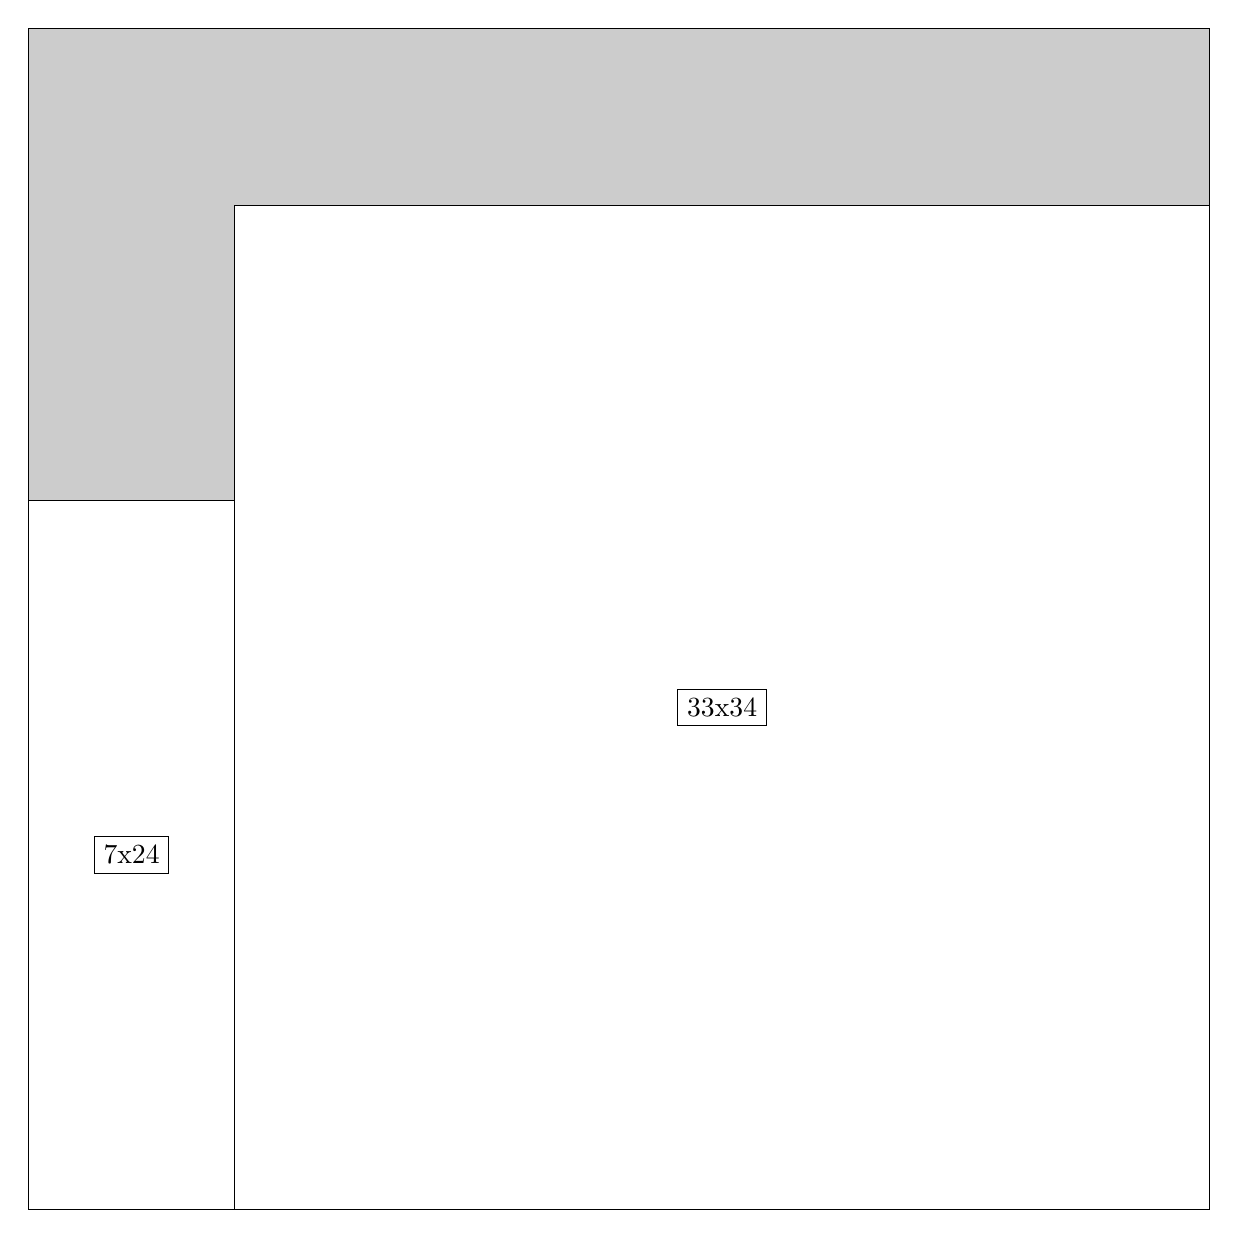
\begin{tikzpicture}[shorten >=1pt,scale=1.0,every node/.style={scale=1.0},->]
\tikzstyle{vertex}=[circle,fill=black!25,minimum size=14pt,inner sep=0pt]
\filldraw[fill=gray!40!white, draw=black] (0,0) rectangle (15.0,15.0);
\foreach \name/\x/\y/\w/\h in {33x34/2.625/0.0/12.375/12.75,7x24/0.0/0.0/2.625/9.0}
\filldraw[fill=white!40!white, draw=black] (\x,\y) rectangle node[draw] (\name) {\name} ++(\w,\h);
\end{tikzpicture}


w =33 , h =34 , x =7 , y =0 , v =1122
\par
w =7 , h =24 , x =0 , y =0 , v =168
\par
\newpage


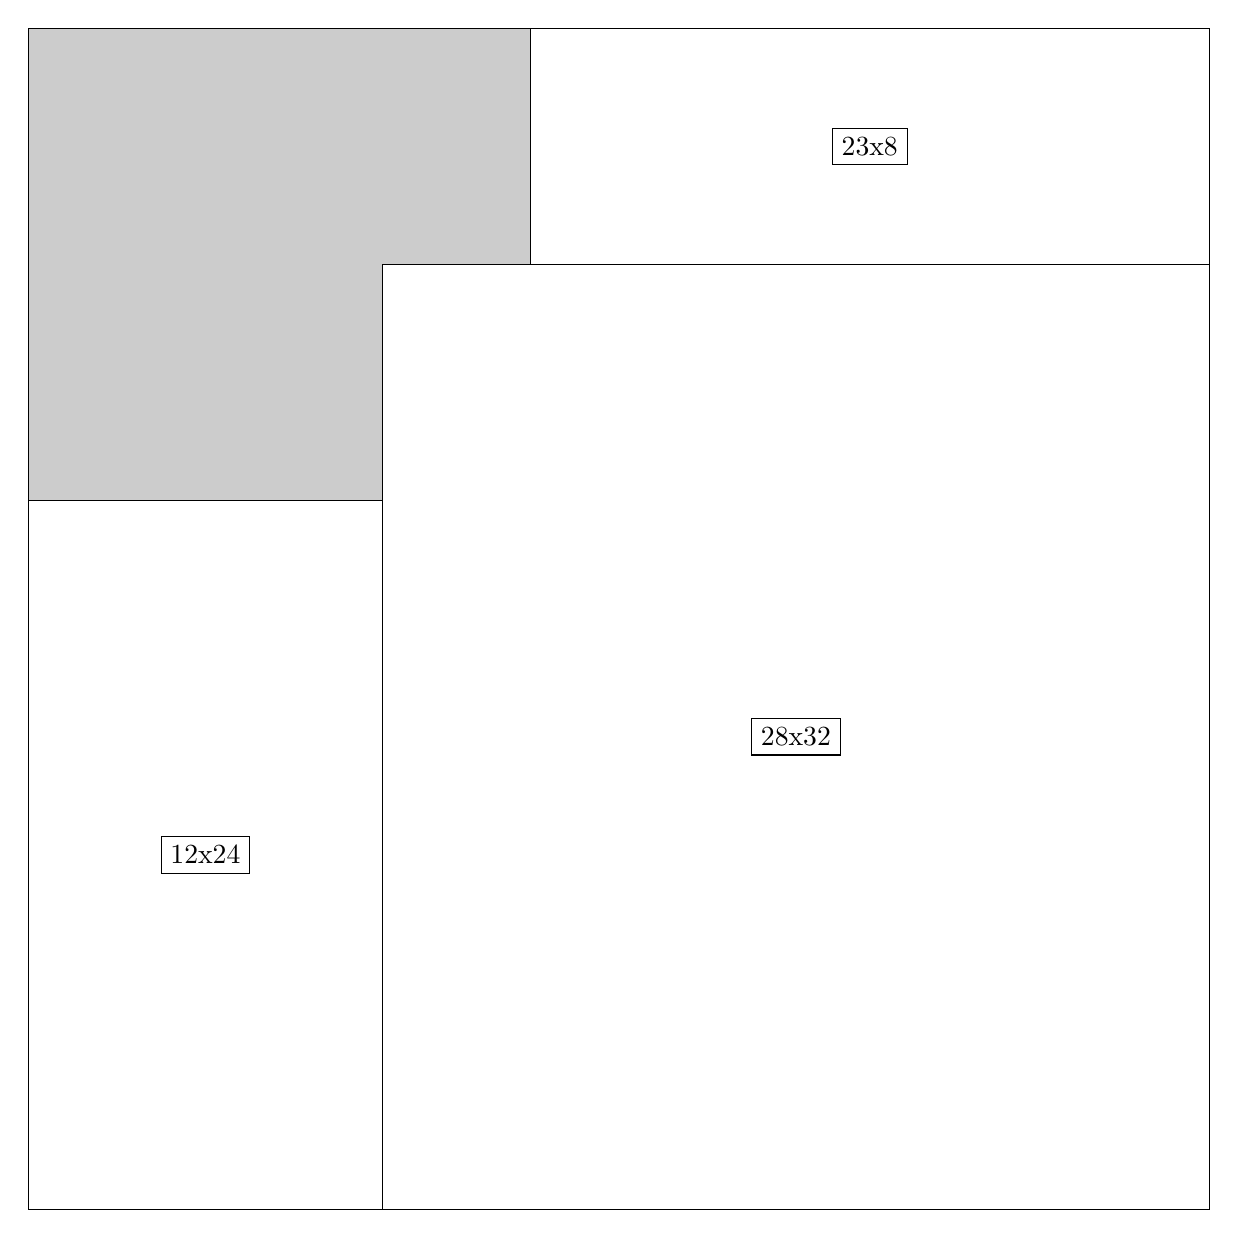
\begin{tikzpicture}[shorten >=1pt,scale=1.0,every node/.style={scale=1.0},->]
\tikzstyle{vertex}=[circle,fill=black!25,minimum size=14pt,inner sep=0pt]
\filldraw[fill=gray!40!white, draw=black] (0,0) rectangle (15.0,15.0);
\foreach \name/\x/\y/\w/\h in {28x32/4.5/0.0/10.5/12.0,12x24/0.0/0.0/4.5/9.0,23x8/6.375/12.0/8.625/3.0}
\filldraw[fill=white!40!white, draw=black] (\x,\y) rectangle node[draw] (\name) {\name} ++(\w,\h);
\end{tikzpicture}


w =28 , h =32 , x =12 , y =0 , v =896
\par
w =12 , h =24 , x =0 , y =0 , v =288
\par
w =23 , h =8 , x =17 , y =32 , v =184
\par
\newpage


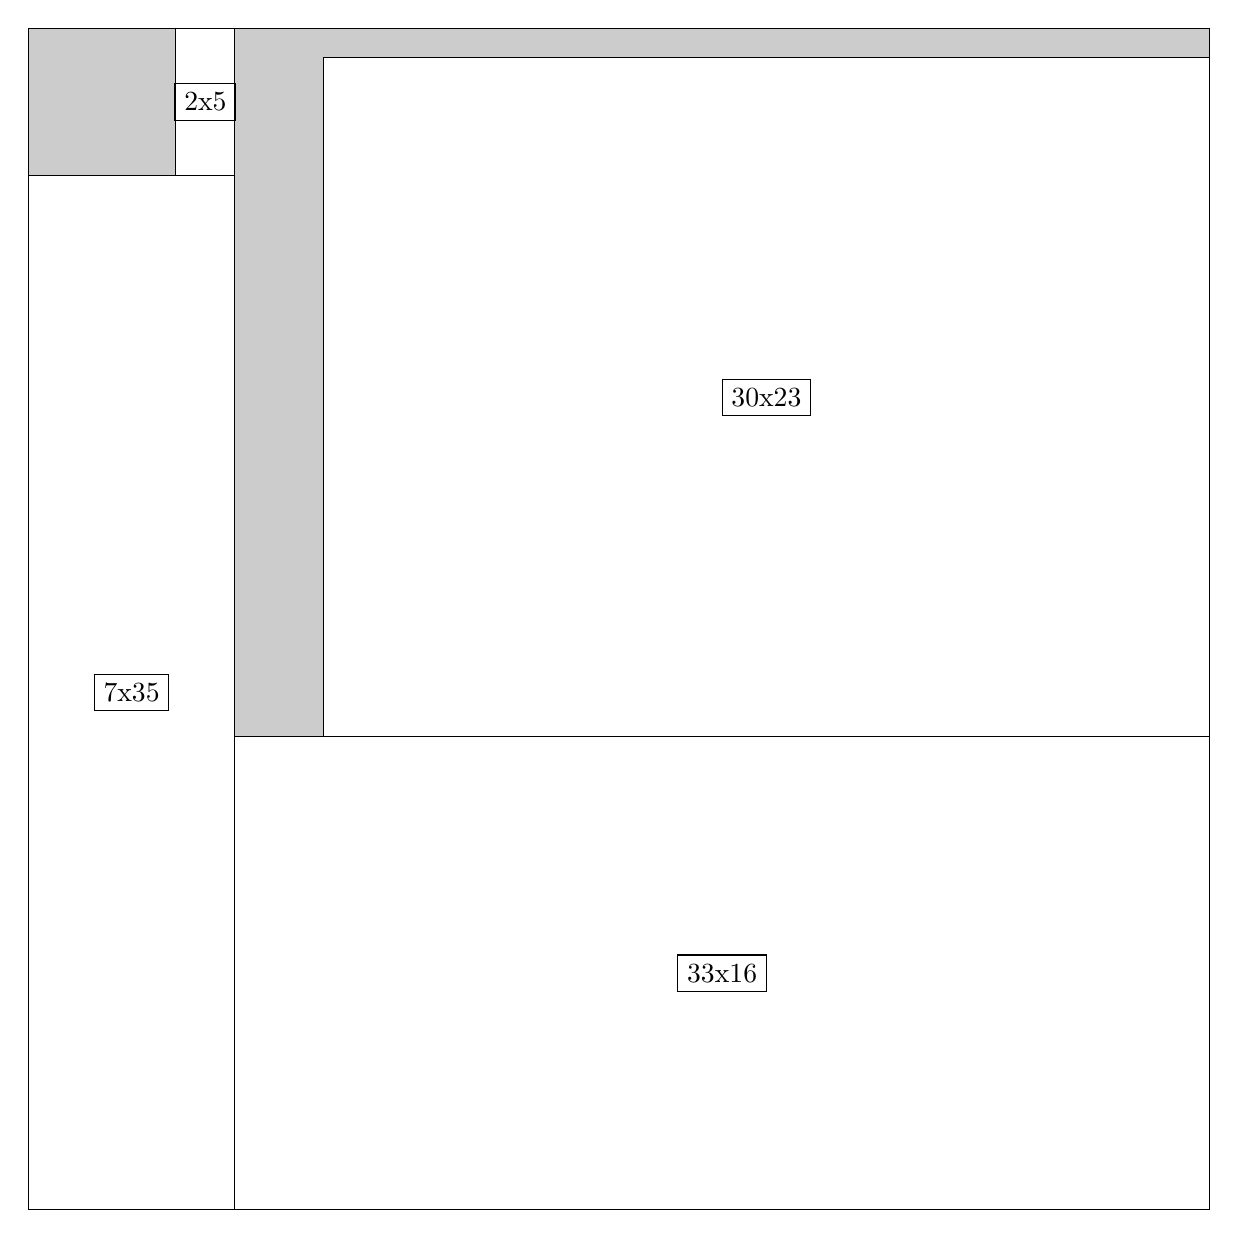
\begin{tikzpicture}[shorten >=1pt,scale=1.0,every node/.style={scale=1.0},->]
\tikzstyle{vertex}=[circle,fill=black!25,minimum size=14pt,inner sep=0pt]
\filldraw[fill=gray!40!white, draw=black] (0,0) rectangle (15.0,15.0);
\foreach \name/\x/\y/\w/\h in {33x16/2.625/0.0/12.375/6.0,30x23/3.75/6.0/11.25/8.625,7x35/0.0/0.0/2.625/13.125,2x5/1.875/13.125/0.75/1.875}
\filldraw[fill=white!40!white, draw=black] (\x,\y) rectangle node[draw] (\name) {\name} ++(\w,\h);
\end{tikzpicture}


w =33 , h =16 , x =7 , y =0 , v =528
\par
w =30 , h =23 , x =10 , y =16 , v =690
\par
w =7 , h =35 , x =0 , y =0 , v =245
\par
w =2 , h =5 , x =5 , y =35 , v =10
\par
\newpage


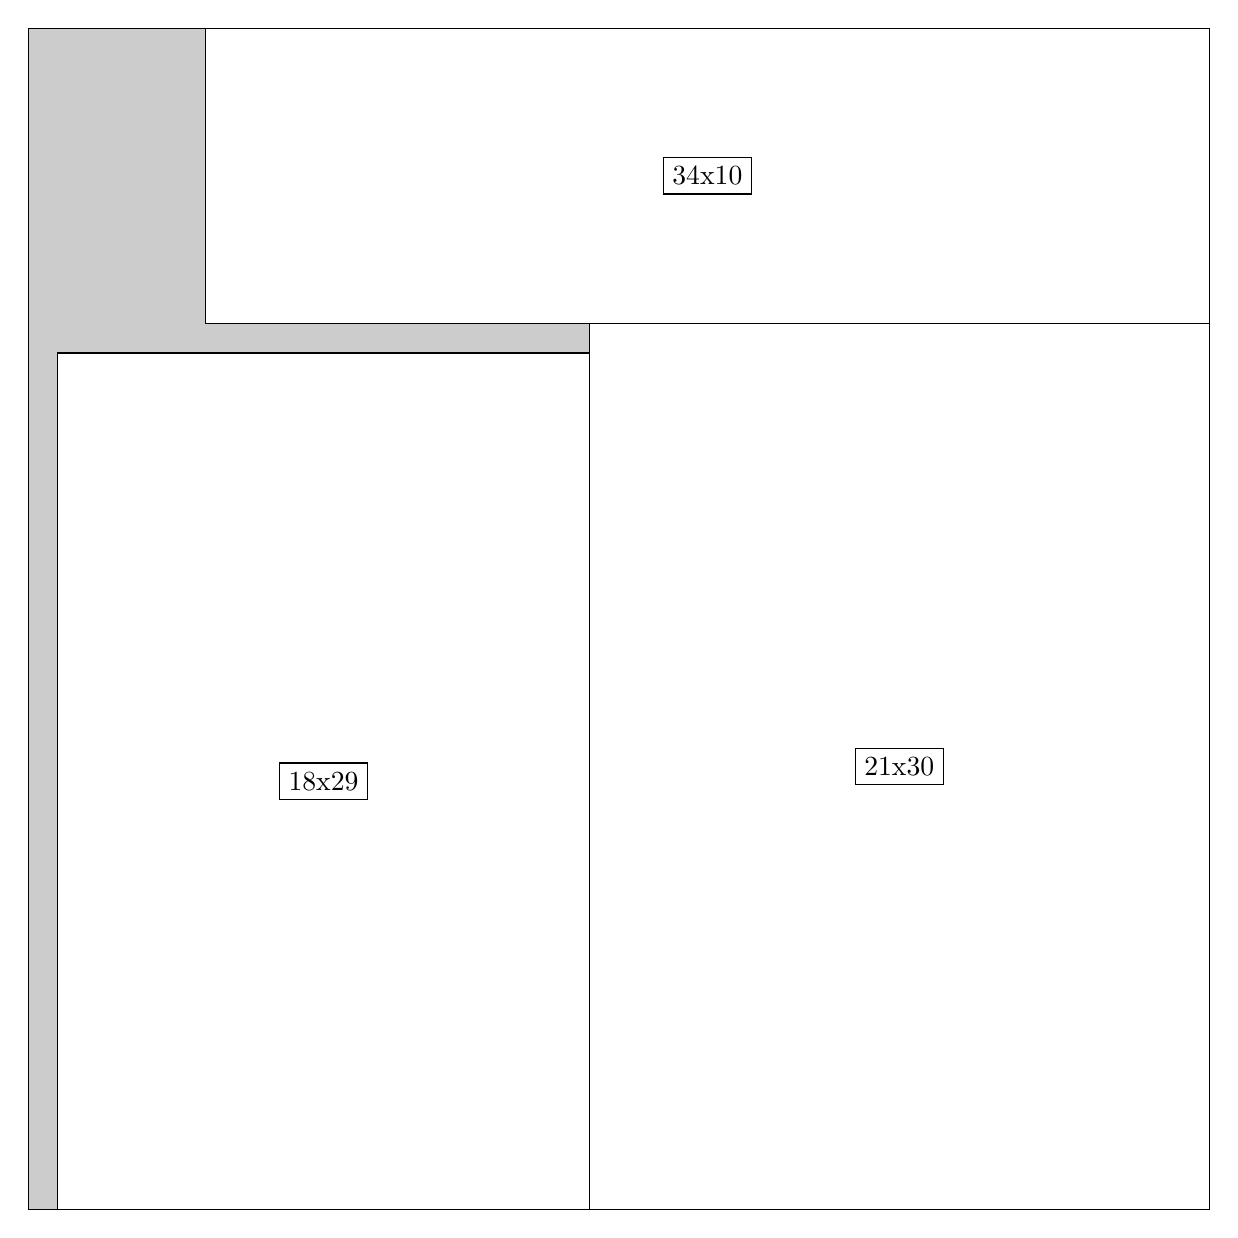
\begin{tikzpicture}[shorten >=1pt,scale=1.0,every node/.style={scale=1.0},->]
\tikzstyle{vertex}=[circle,fill=black!25,minimum size=14pt,inner sep=0pt]
\filldraw[fill=gray!40!white, draw=black] (0,0) rectangle (15.0,15.0);
\foreach \name/\x/\y/\w/\h in {21x30/7.125/0.0/7.875/11.25,18x29/0.375/0.0/6.75/10.875,34x10/2.25/11.25/12.75/3.75}
\filldraw[fill=white!40!white, draw=black] (\x,\y) rectangle node[draw] (\name) {\name} ++(\w,\h);
\end{tikzpicture}


w =21 , h =30 , x =19 , y =0 , v =630
\par
w =18 , h =29 , x =1 , y =0 , v =522
\par
w =34 , h =10 , x =6 , y =30 , v =340
\par
\newpage


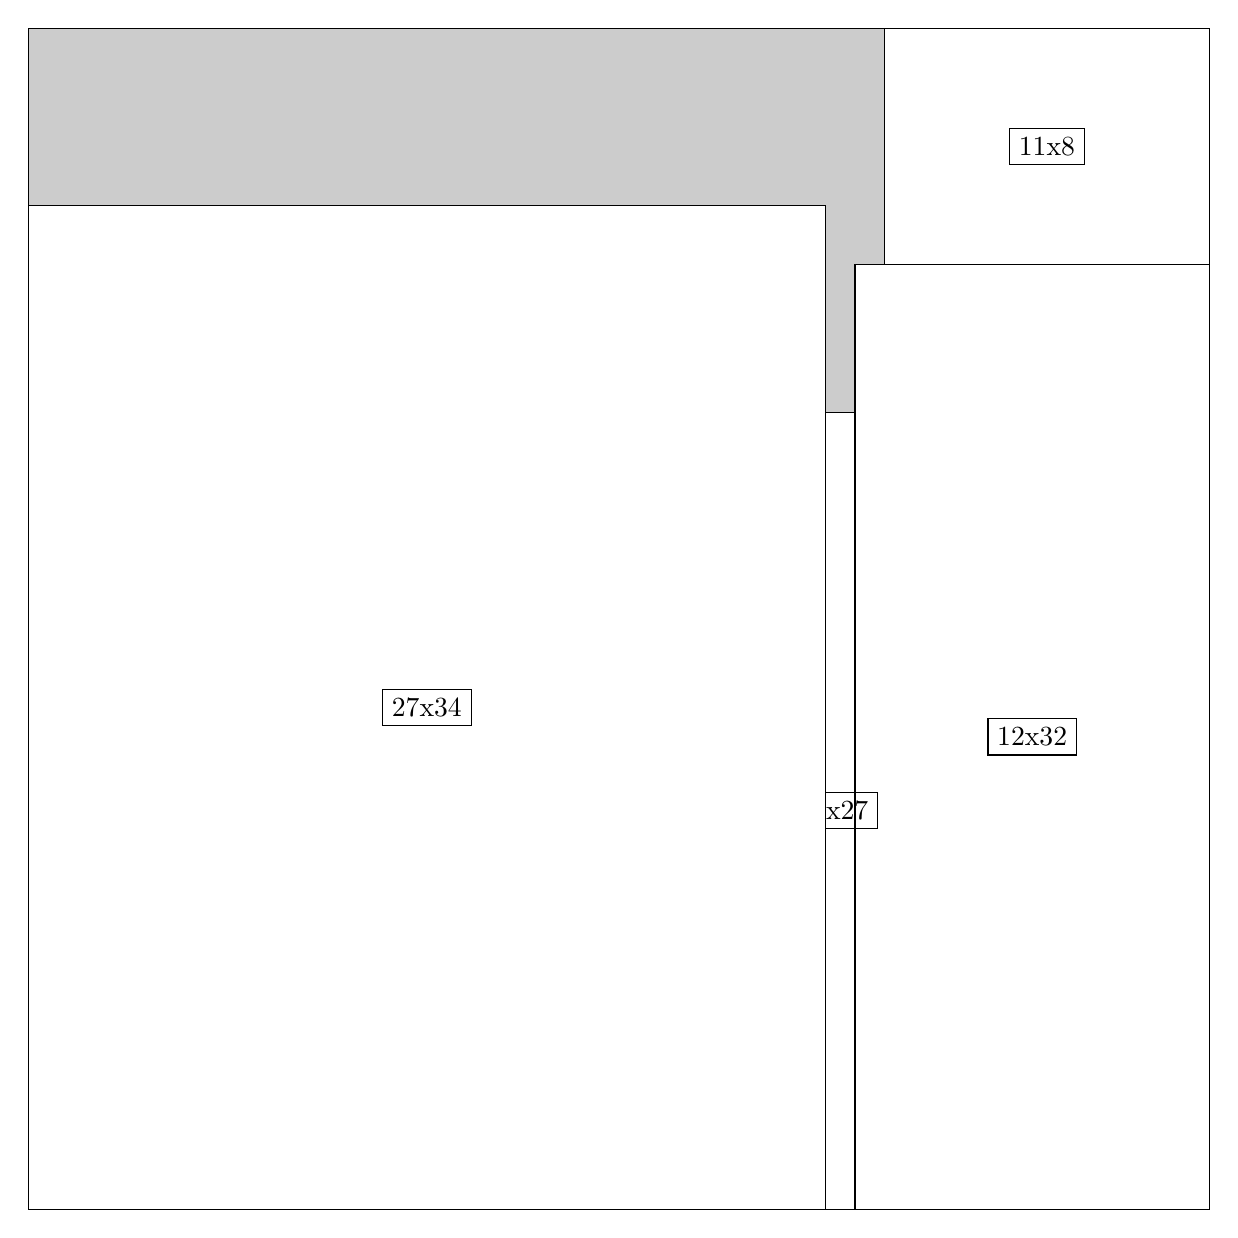
\begin{tikzpicture}[shorten >=1pt,scale=1.0,every node/.style={scale=1.0},->]
\tikzstyle{vertex}=[circle,fill=black!25,minimum size=14pt,inner sep=0pt]
\filldraw[fill=gray!40!white, draw=black] (0,0) rectangle (15.0,15.0);
\foreach \name/\x/\y/\w/\h in {12x32/10.5/0.0/4.5/12.0,1x27/10.125/0.0/0.375/10.125,11x8/10.875/12.0/4.125/3.0,27x34/0.0/0.0/10.125/12.75}
\filldraw[fill=white!40!white, draw=black] (\x,\y) rectangle node[draw] (\name) {\name} ++(\w,\h);
\end{tikzpicture}


w =12 , h =32 , x =28 , y =0 , v =384
\par
w =1 , h =27 , x =27 , y =0 , v =27
\par
w =11 , h =8 , x =29 , y =32 , v =88
\par
w =27 , h =34 , x =0 , y =0 , v =918
\par
\newpage


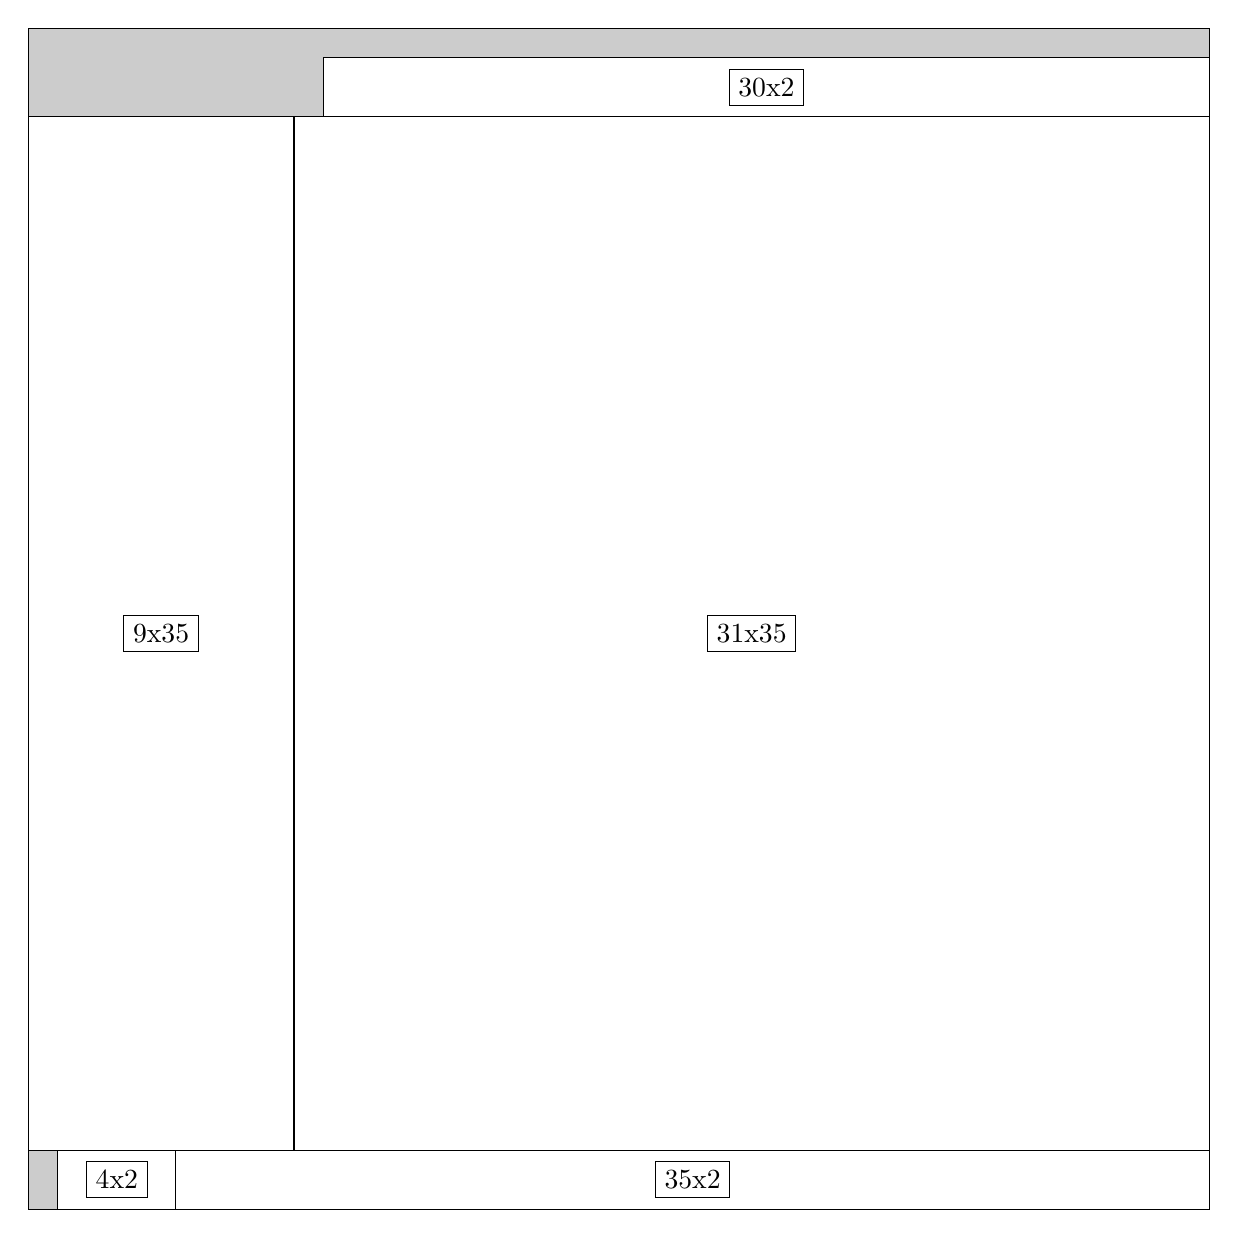
\begin{tikzpicture}[shorten >=1pt,scale=1.0,every node/.style={scale=1.0},->]
\tikzstyle{vertex}=[circle,fill=black!25,minimum size=14pt,inner sep=0pt]
\filldraw[fill=gray!40!white, draw=black] (0,0) rectangle (15.0,15.0);
\foreach \name/\x/\y/\w/\h in {35x2/1.875/0.0/13.125/0.75,4x2/0.375/0.0/1.5/0.75,31x35/3.375/0.75/11.625/13.125,30x2/3.75/13.875/11.25/0.75,9x35/0.0/0.75/3.375/13.125}
\filldraw[fill=white!40!white, draw=black] (\x,\y) rectangle node[draw] (\name) {\name} ++(\w,\h);
\end{tikzpicture}


w =35 , h =2 , x =5 , y =0 , v =70
\par
w =4 , h =2 , x =1 , y =0 , v =8
\par
w =31 , h =35 , x =9 , y =2 , v =1085
\par
w =30 , h =2 , x =10 , y =37 , v =60
\par
w =9 , h =35 , x =0 , y =2 , v =315
\par
\newpage


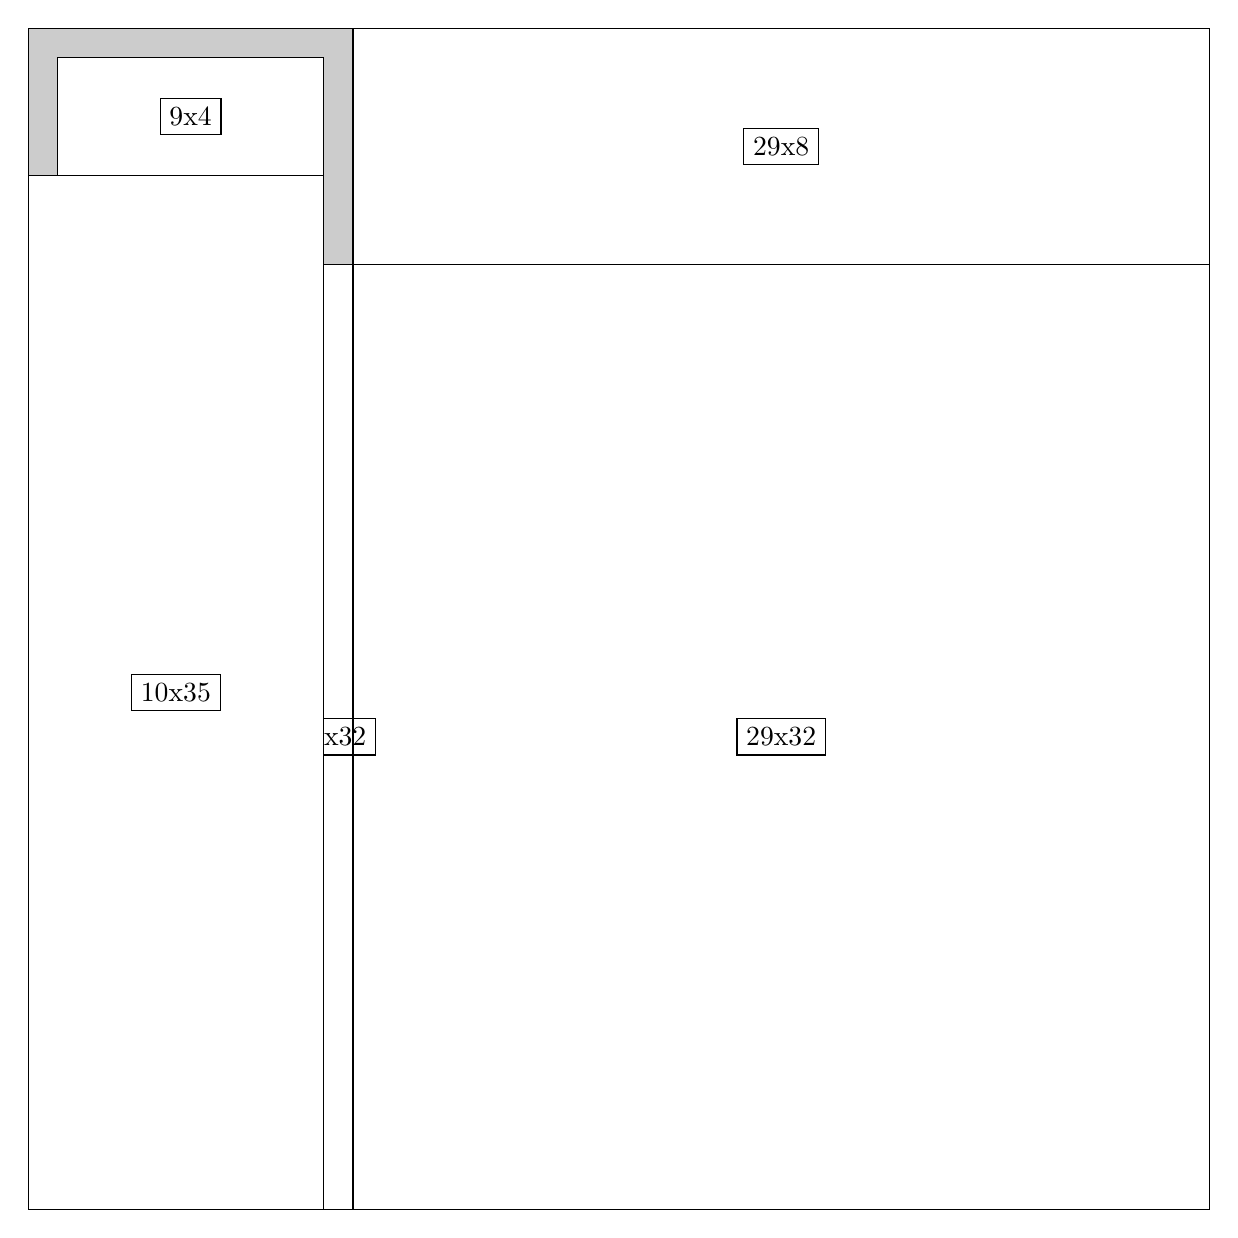
\begin{tikzpicture}[shorten >=1pt,scale=1.0,every node/.style={scale=1.0},->]
\tikzstyle{vertex}=[circle,fill=black!25,minimum size=14pt,inner sep=0pt]
\filldraw[fill=gray!40!white, draw=black] (0,0) rectangle (15.0,15.0);
\foreach \name/\x/\y/\w/\h in {29x32/4.125/0.0/10.875/12.0,1x32/3.75/0.0/0.375/12.0,29x8/4.125/12.0/10.875/3.0,10x35/0.0/0.0/3.75/13.125,9x4/0.375/13.125/3.375/1.5}
\filldraw[fill=white!40!white, draw=black] (\x,\y) rectangle node[draw] (\name) {\name} ++(\w,\h);
\end{tikzpicture}


w =29 , h =32 , x =11 , y =0 , v =928
\par
w =1 , h =32 , x =10 , y =0 , v =32
\par
w =29 , h =8 , x =11 , y =32 , v =232
\par
w =10 , h =35 , x =0 , y =0 , v =350
\par
w =9 , h =4 , x =1 , y =35 , v =36
\par
\newpage


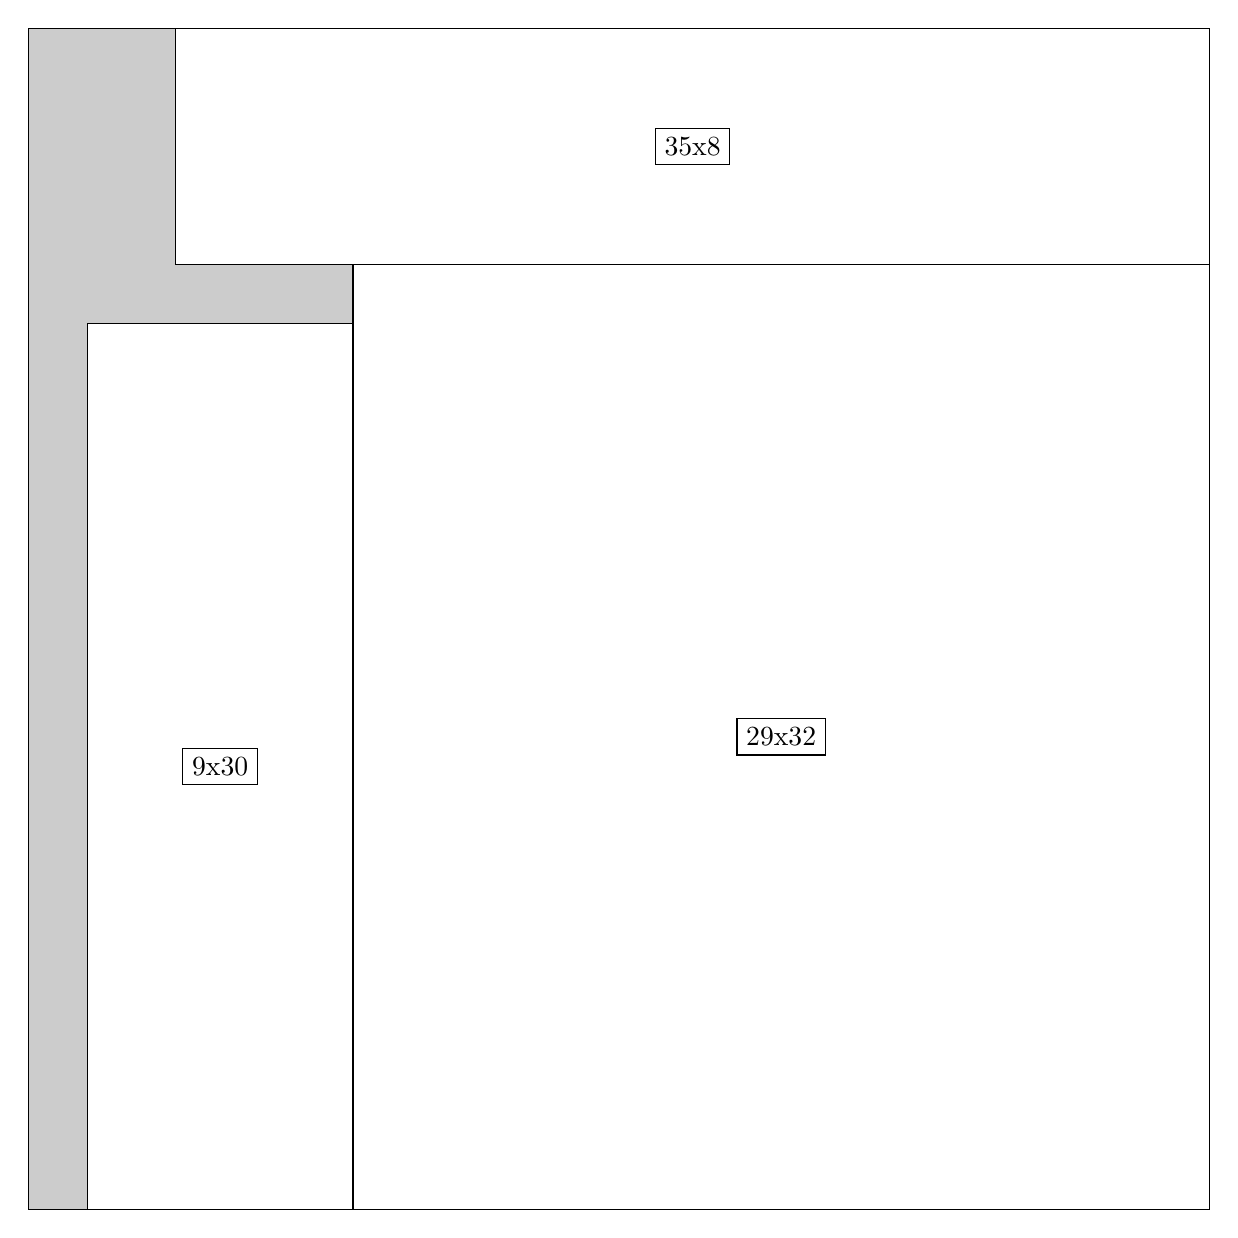
\begin{tikzpicture}[shorten >=1pt,scale=1.0,every node/.style={scale=1.0},->]
\tikzstyle{vertex}=[circle,fill=black!25,minimum size=14pt,inner sep=0pt]
\filldraw[fill=gray!40!white, draw=black] (0,0) rectangle (15.0,15.0);
\foreach \name/\x/\y/\w/\h in {29x32/4.125/0.0/10.875/12.0,9x30/0.75/0.0/3.375/11.25,35x8/1.875/12.0/13.125/3.0}
\filldraw[fill=white!40!white, draw=black] (\x,\y) rectangle node[draw] (\name) {\name} ++(\w,\h);
\end{tikzpicture}


w =29 , h =32 , x =11 , y =0 , v =928
\par
w =9 , h =30 , x =2 , y =0 , v =270
\par
w =35 , h =8 , x =5 , y =32 , v =280
\par
\newpage


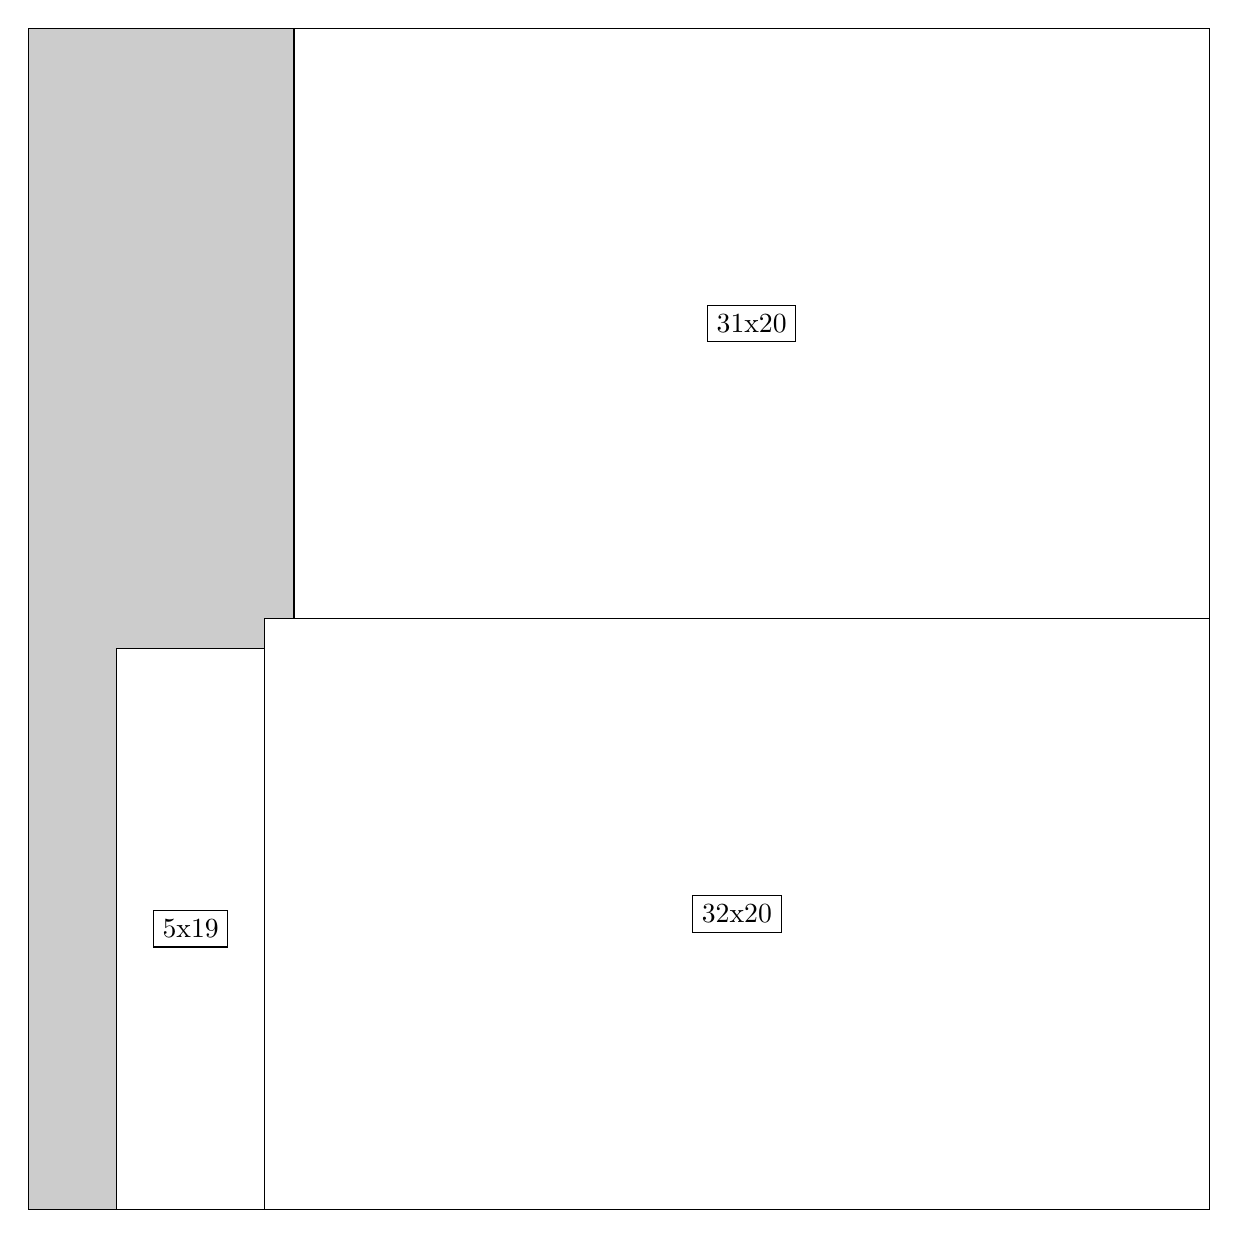
\begin{tikzpicture}[shorten >=1pt,scale=1.0,every node/.style={scale=1.0},->]
\tikzstyle{vertex}=[circle,fill=black!25,minimum size=14pt,inner sep=0pt]
\filldraw[fill=gray!40!white, draw=black] (0,0) rectangle (15.0,15.0);
\foreach \name/\x/\y/\w/\h in {32x20/3.0/0.0/12.0/7.5,5x19/1.125/0.0/1.875/7.125,31x20/3.375/7.5/11.625/7.5}
\filldraw[fill=white!40!white, draw=black] (\x,\y) rectangle node[draw] (\name) {\name} ++(\w,\h);
\end{tikzpicture}


w =32 , h =20 , x =8 , y =0 , v =640
\par
w =5 , h =19 , x =3 , y =0 , v =95
\par
w =31 , h =20 , x =9 , y =20 , v =620
\par
\newpage


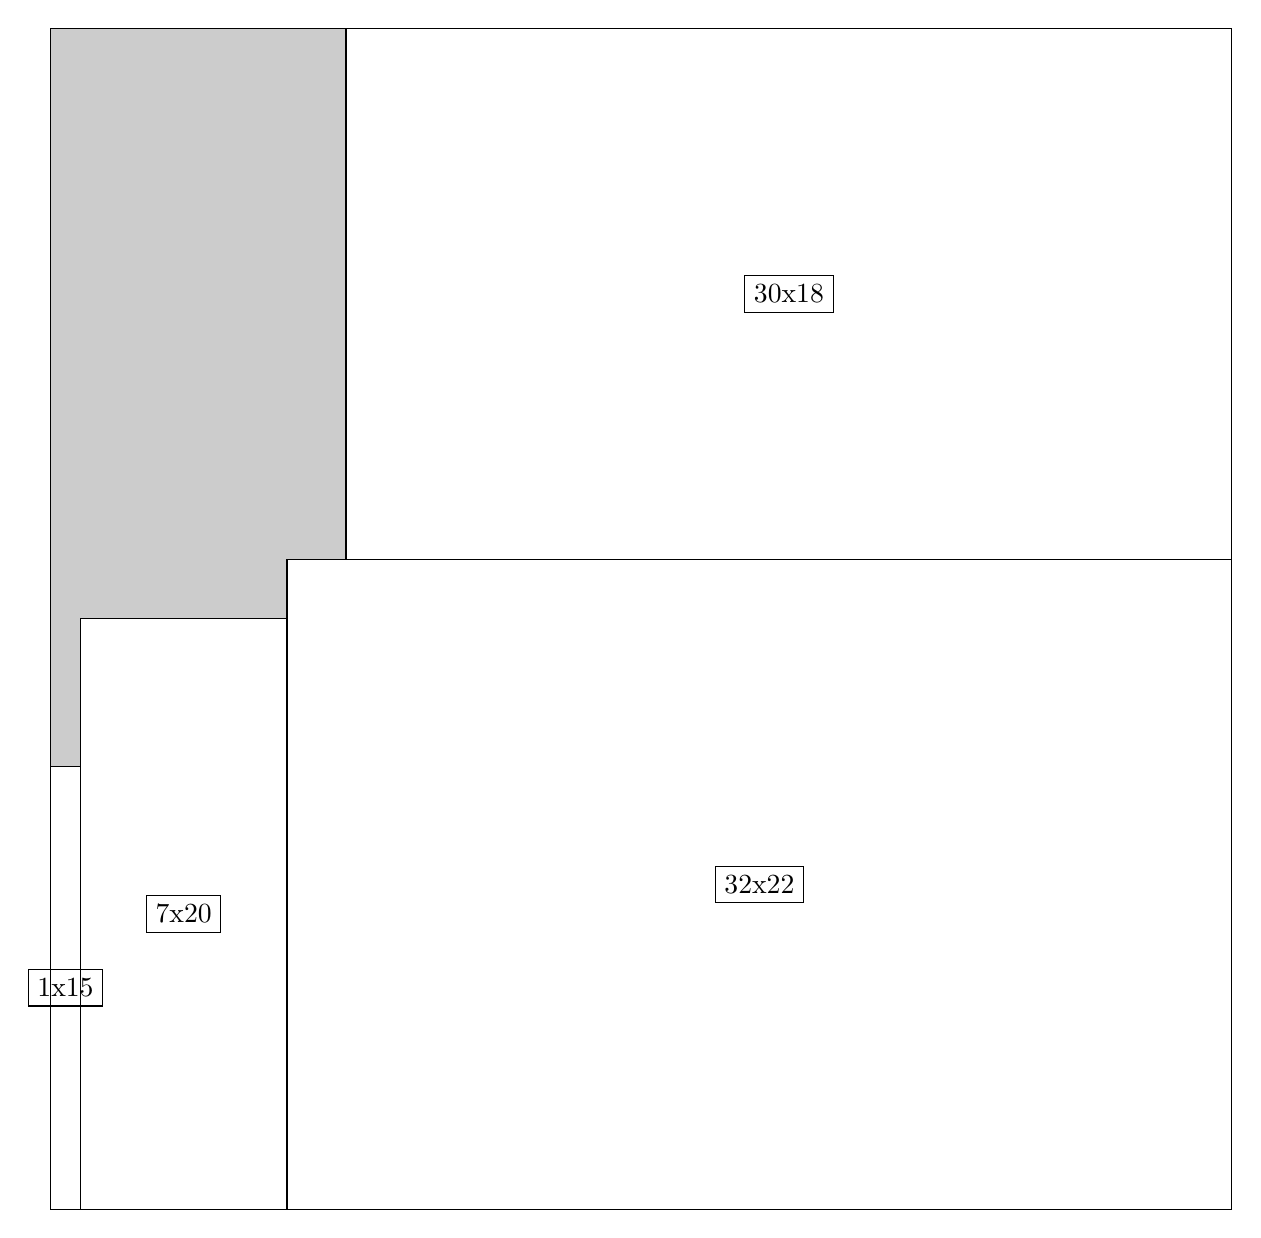
\begin{tikzpicture}[shorten >=1pt,scale=1.0,every node/.style={scale=1.0},->]
\tikzstyle{vertex}=[circle,fill=black!25,minimum size=14pt,inner sep=0pt]
\filldraw[fill=gray!40!white, draw=black] (0,0) rectangle (15.0,15.0);
\foreach \name/\x/\y/\w/\h in {32x22/3.0/0.0/12.0/8.25,7x20/0.375/0.0/2.625/7.5,1x15/0.0/0.0/0.375/5.625,30x18/3.75/8.25/11.25/6.75}
\filldraw[fill=white!40!white, draw=black] (\x,\y) rectangle node[draw] (\name) {\name} ++(\w,\h);
\end{tikzpicture}


w =32 , h =22 , x =8 , y =0 , v =704
\par
w =7 , h =20 , x =1 , y =0 , v =140
\par
w =1 , h =15 , x =0 , y =0 , v =15
\par
w =30 , h =18 , x =10 , y =22 , v =540
\par
\newpage


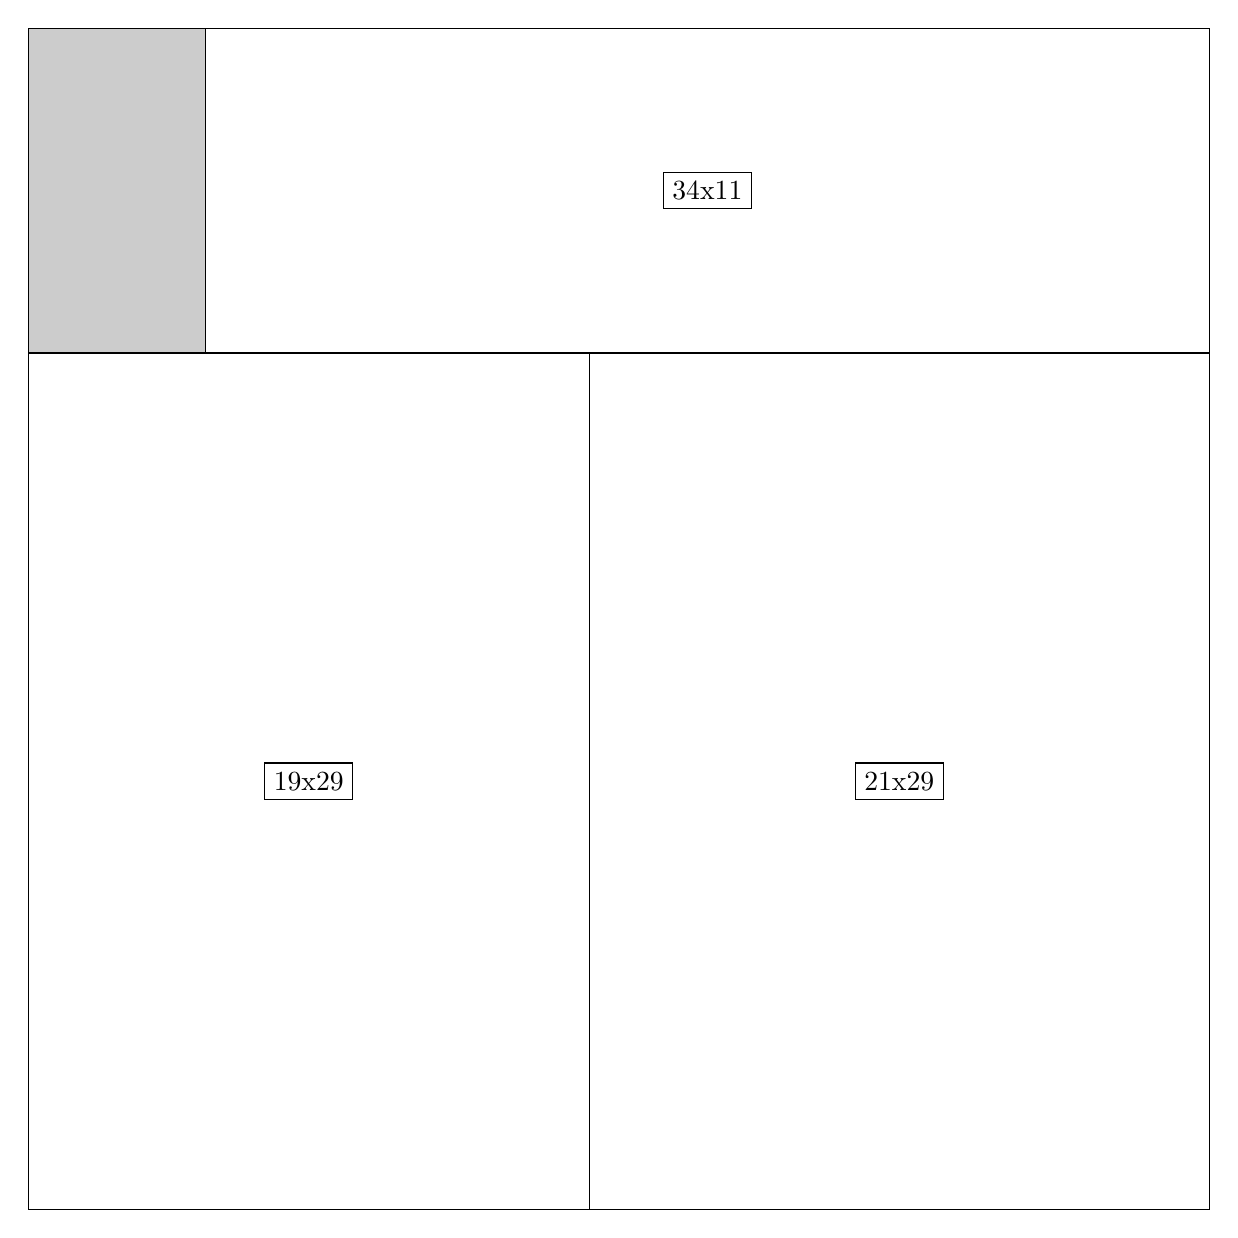
\begin{tikzpicture}[shorten >=1pt,scale=1.0,every node/.style={scale=1.0},->]
\tikzstyle{vertex}=[circle,fill=black!25,minimum size=14pt,inner sep=0pt]
\filldraw[fill=gray!40!white, draw=black] (0,0) rectangle (15.0,15.0);
\foreach \name/\x/\y/\w/\h in {21x29/7.125/0.0/7.875/10.875,19x29/0.0/0.0/7.125/10.875,34x11/2.25/10.875/12.75/4.125}
\filldraw[fill=white!40!white, draw=black] (\x,\y) rectangle node[draw] (\name) {\name} ++(\w,\h);
\end{tikzpicture}


w =21 , h =29 , x =19 , y =0 , v =609
\par
w =19 , h =29 , x =0 , y =0 , v =551
\par
w =34 , h =11 , x =6 , y =29 , v =374
\par
\newpage


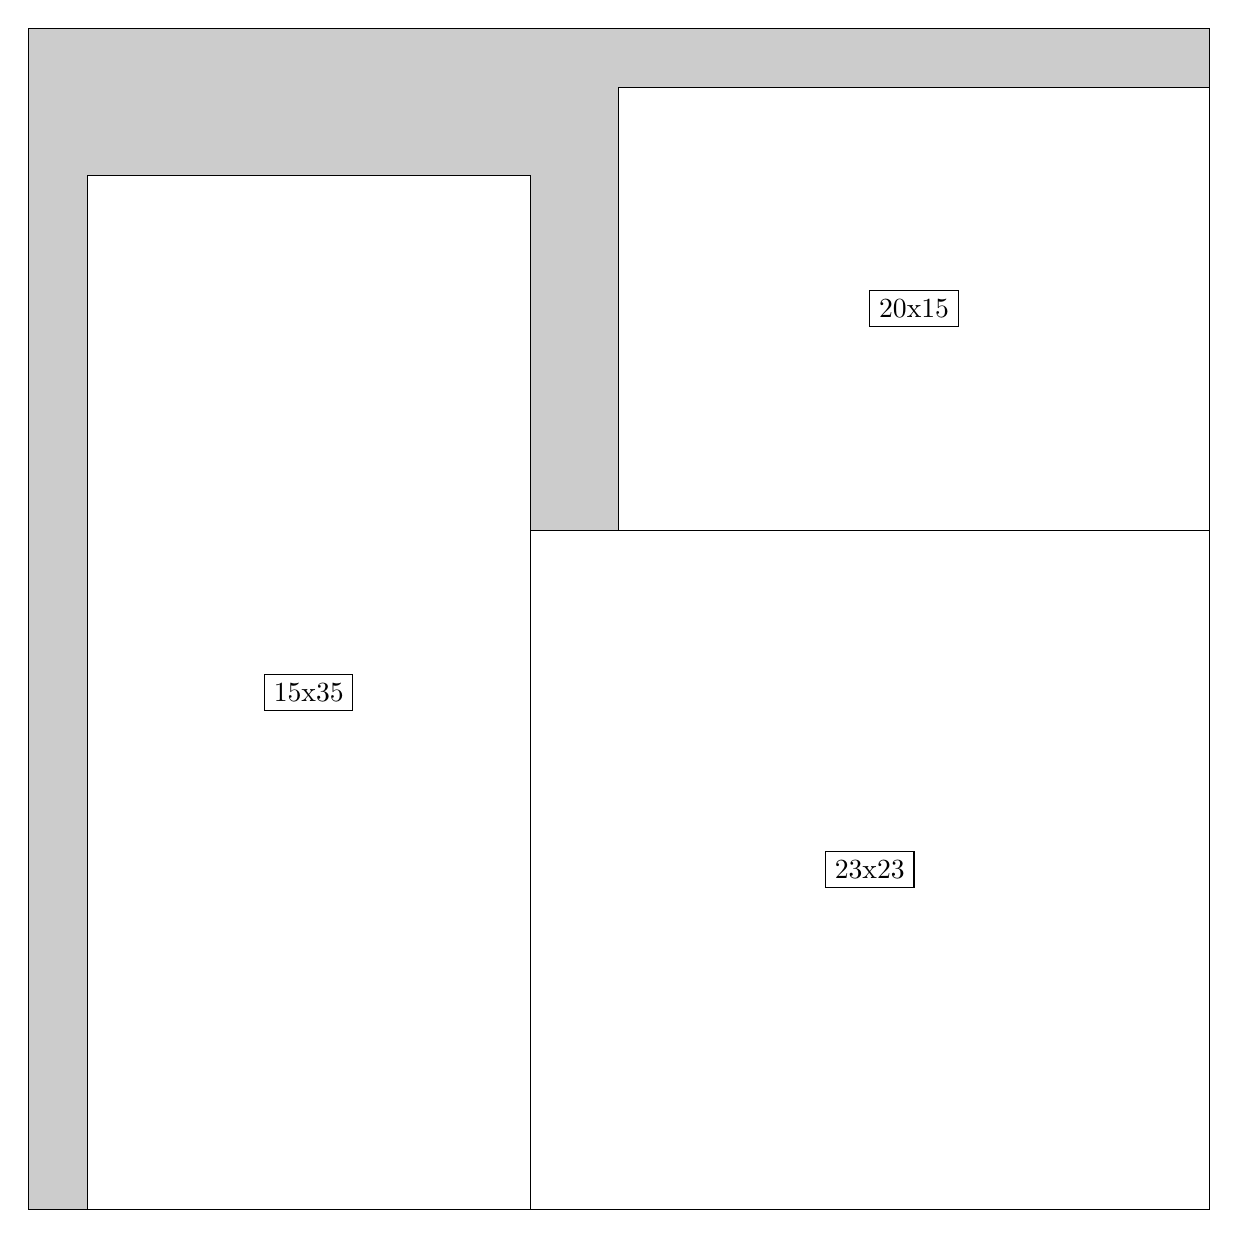
\begin{tikzpicture}[shorten >=1pt,scale=1.0,every node/.style={scale=1.0},->]
\tikzstyle{vertex}=[circle,fill=black!25,minimum size=14pt,inner sep=0pt]
\filldraw[fill=gray!40!white, draw=black] (0,0) rectangle (15.0,15.0);
\foreach \name/\x/\y/\w/\h in {23x23/6.375/0.0/8.625/8.625,20x15/7.5/8.625/7.5/5.625,15x35/0.75/0.0/5.625/13.125}
\filldraw[fill=white!40!white, draw=black] (\x,\y) rectangle node[draw] (\name) {\name} ++(\w,\h);
\end{tikzpicture}


w =23 , h =23 , x =17 , y =0 , v =529
\par
w =20 , h =15 , x =20 , y =23 , v =300
\par
w =15 , h =35 , x =2 , y =0 , v =525
\par
\newpage


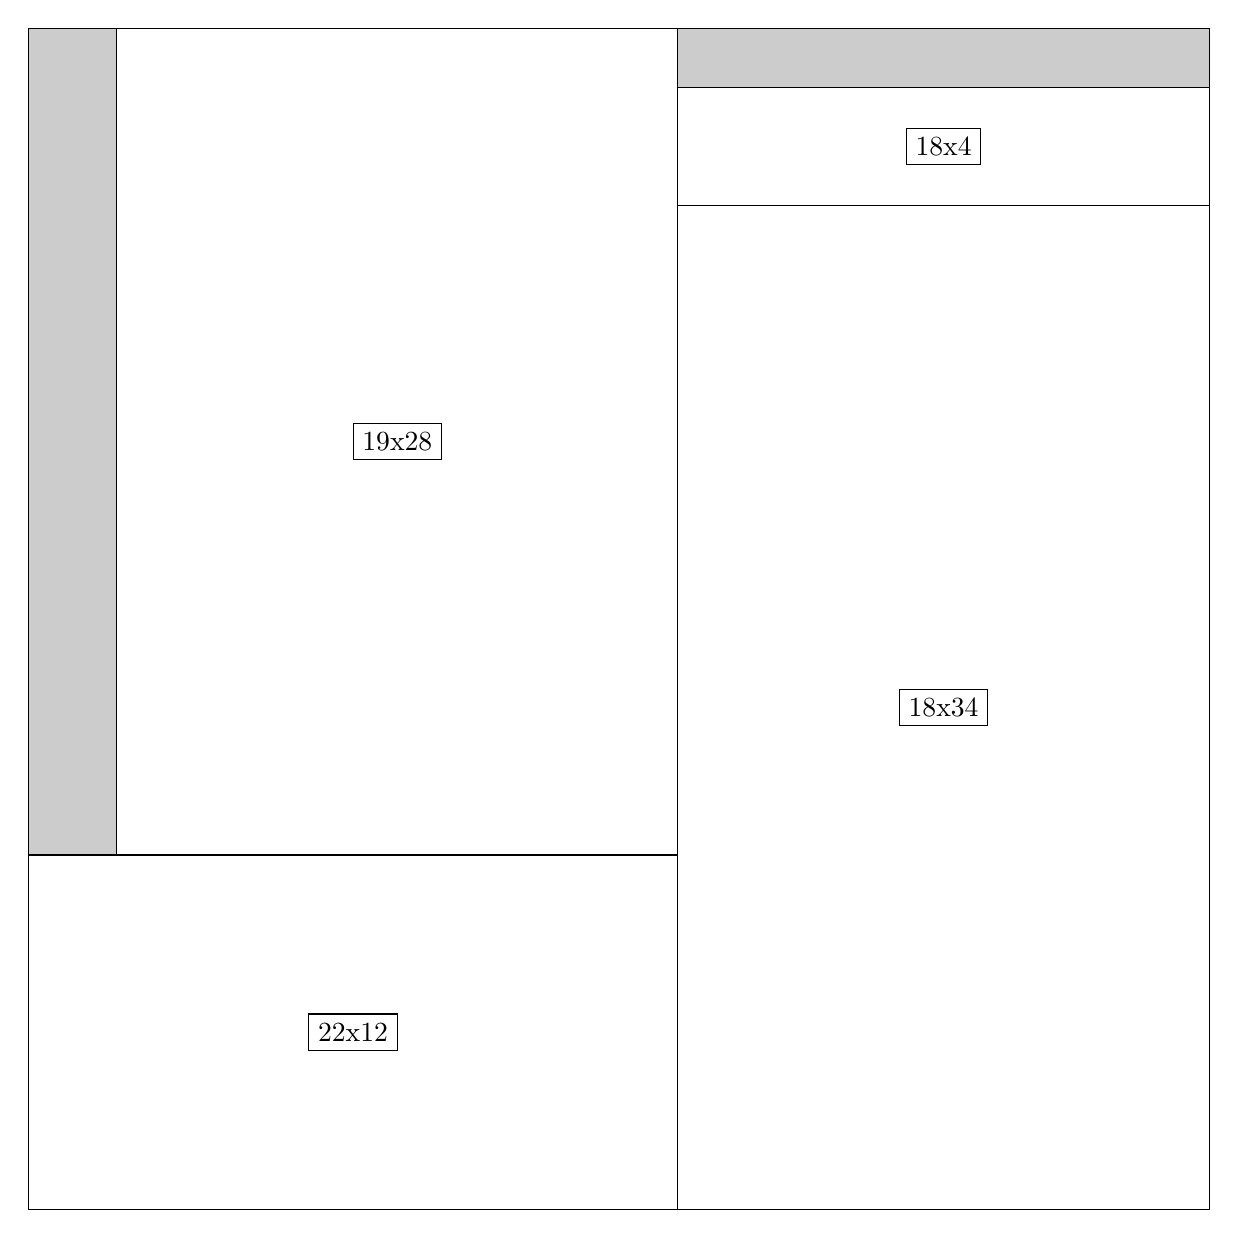
\begin{tikzpicture}[shorten >=1pt,scale=1.0,every node/.style={scale=1.0},->]
\tikzstyle{vertex}=[circle,fill=black!25,minimum size=14pt,inner sep=0pt]
\filldraw[fill=gray!40!white, draw=black] (0,0) rectangle (15.0,15.0);
\foreach \name/\x/\y/\w/\h in {18x34/8.25/0.0/6.75/12.75,18x4/8.25/12.75/6.75/1.5,22x12/0.0/0.0/8.25/4.5,19x28/1.125/4.5/7.125/10.5}
\filldraw[fill=white!40!white, draw=black] (\x,\y) rectangle node[draw] (\name) {\name} ++(\w,\h);
\end{tikzpicture}


w =18 , h =34 , x =22 , y =0 , v =612
\par
w =18 , h =4 , x =22 , y =34 , v =72
\par
w =22 , h =12 , x =0 , y =0 , v =264
\par
w =19 , h =28 , x =3 , y =12 , v =532
\par
\newpage


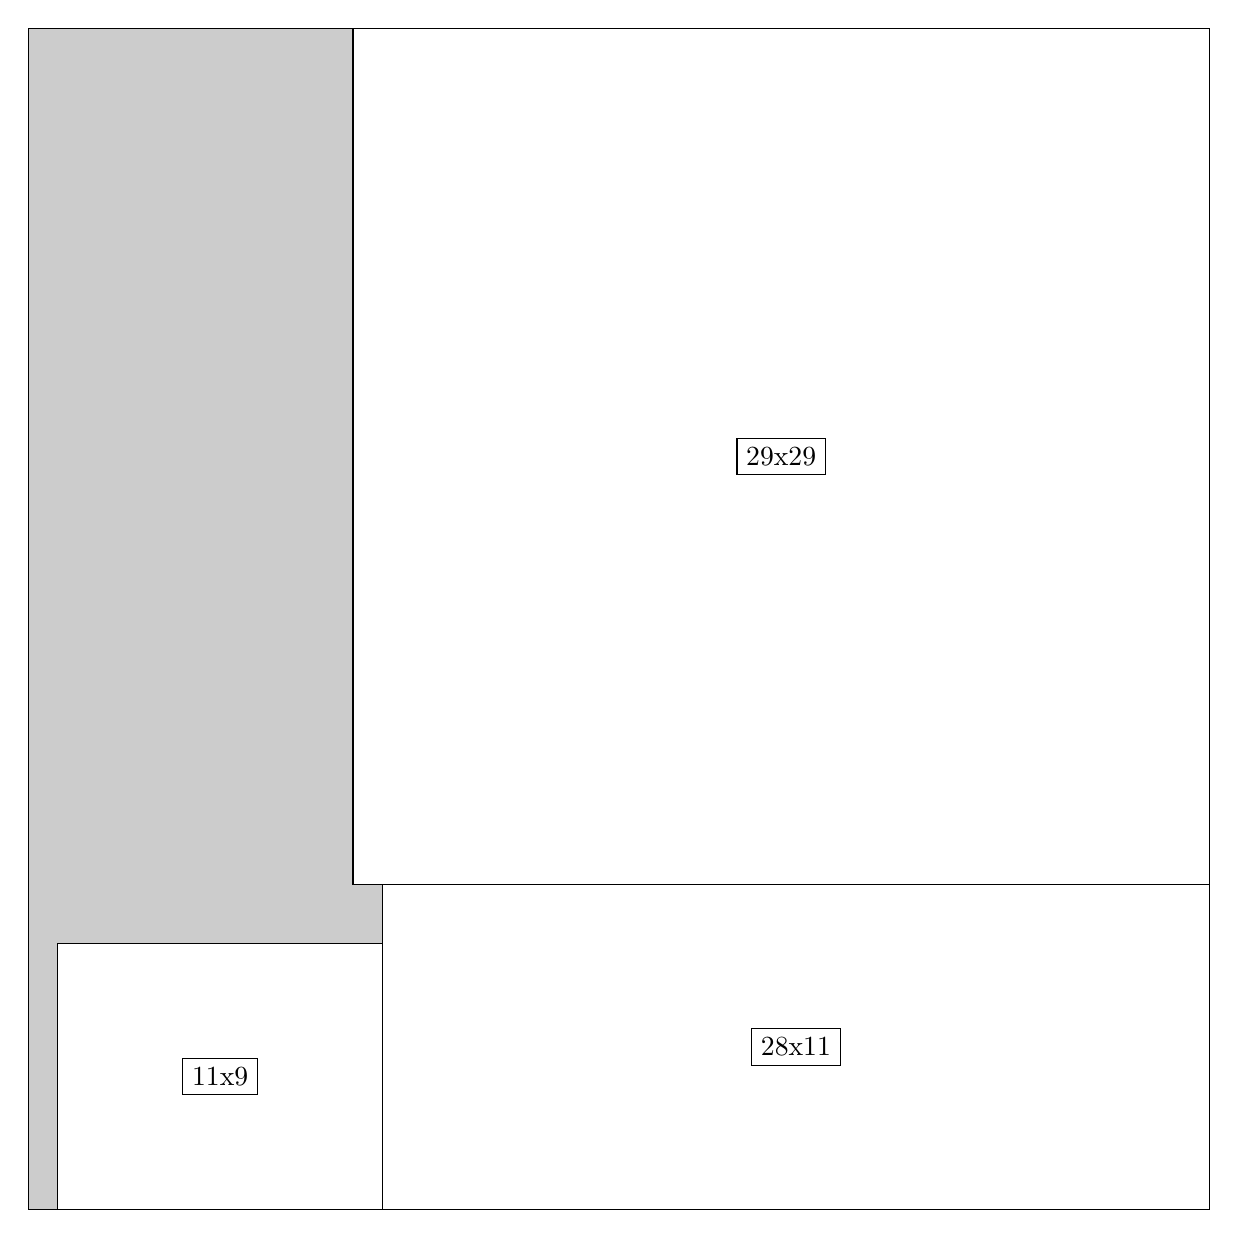
\begin{tikzpicture}[shorten >=1pt,scale=1.0,every node/.style={scale=1.0},->]
\tikzstyle{vertex}=[circle,fill=black!25,minimum size=14pt,inner sep=0pt]
\filldraw[fill=gray!40!white, draw=black] (0,0) rectangle (15.0,15.0);
\foreach \name/\x/\y/\w/\h in {28x11/4.5/0.0/10.5/4.125,11x9/0.375/0.0/4.125/3.375,29x29/4.125/4.125/10.875/10.875}
\filldraw[fill=white!40!white, draw=black] (\x,\y) rectangle node[draw] (\name) {\name} ++(\w,\h);
\end{tikzpicture}


w =28 , h =11 , x =12 , y =0 , v =308
\par
w =11 , h =9 , x =1 , y =0 , v =99
\par
w =29 , h =29 , x =11 , y =11 , v =841
\par
\newpage


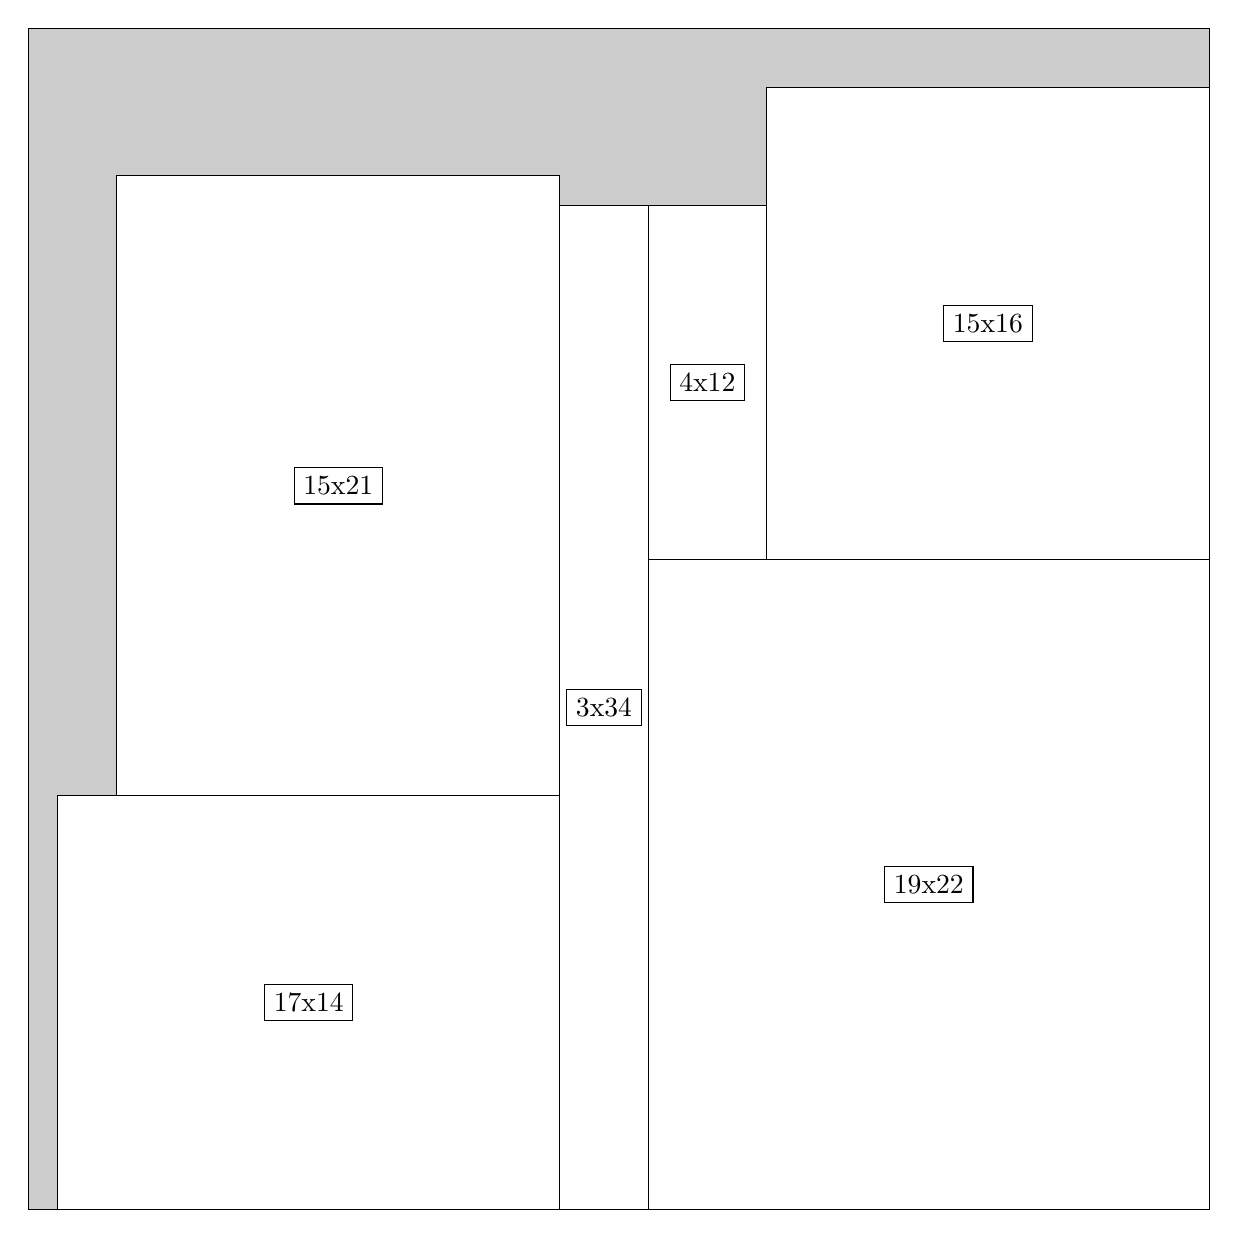
\begin{tikzpicture}[shorten >=1pt,scale=1.0,every node/.style={scale=1.0},->]
\tikzstyle{vertex}=[circle,fill=black!25,minimum size=14pt,inner sep=0pt]
\filldraw[fill=gray!40!white, draw=black] (0,0) rectangle (15.0,15.0);
\foreach \name/\x/\y/\w/\h in {19x22/7.875/0.0/7.125/8.25,15x16/9.375/8.25/5.625/6.0,4x12/7.875/8.25/1.5/4.5,3x34/6.75/0.0/1.125/12.75,17x14/0.375/0.0/6.375/5.25,15x21/1.125/5.25/5.625/7.875}
\filldraw[fill=white!40!white, draw=black] (\x,\y) rectangle node[draw] (\name) {\name} ++(\w,\h);
\end{tikzpicture}


w =19 , h =22 , x =21 , y =0 , v =418
\par
w =15 , h =16 , x =25 , y =22 , v =240
\par
w =4 , h =12 , x =21 , y =22 , v =48
\par
w =3 , h =34 , x =18 , y =0 , v =102
\par
w =17 , h =14 , x =1 , y =0 , v =238
\par
w =15 , h =21 , x =3 , y =14 , v =315
\par
\newpage


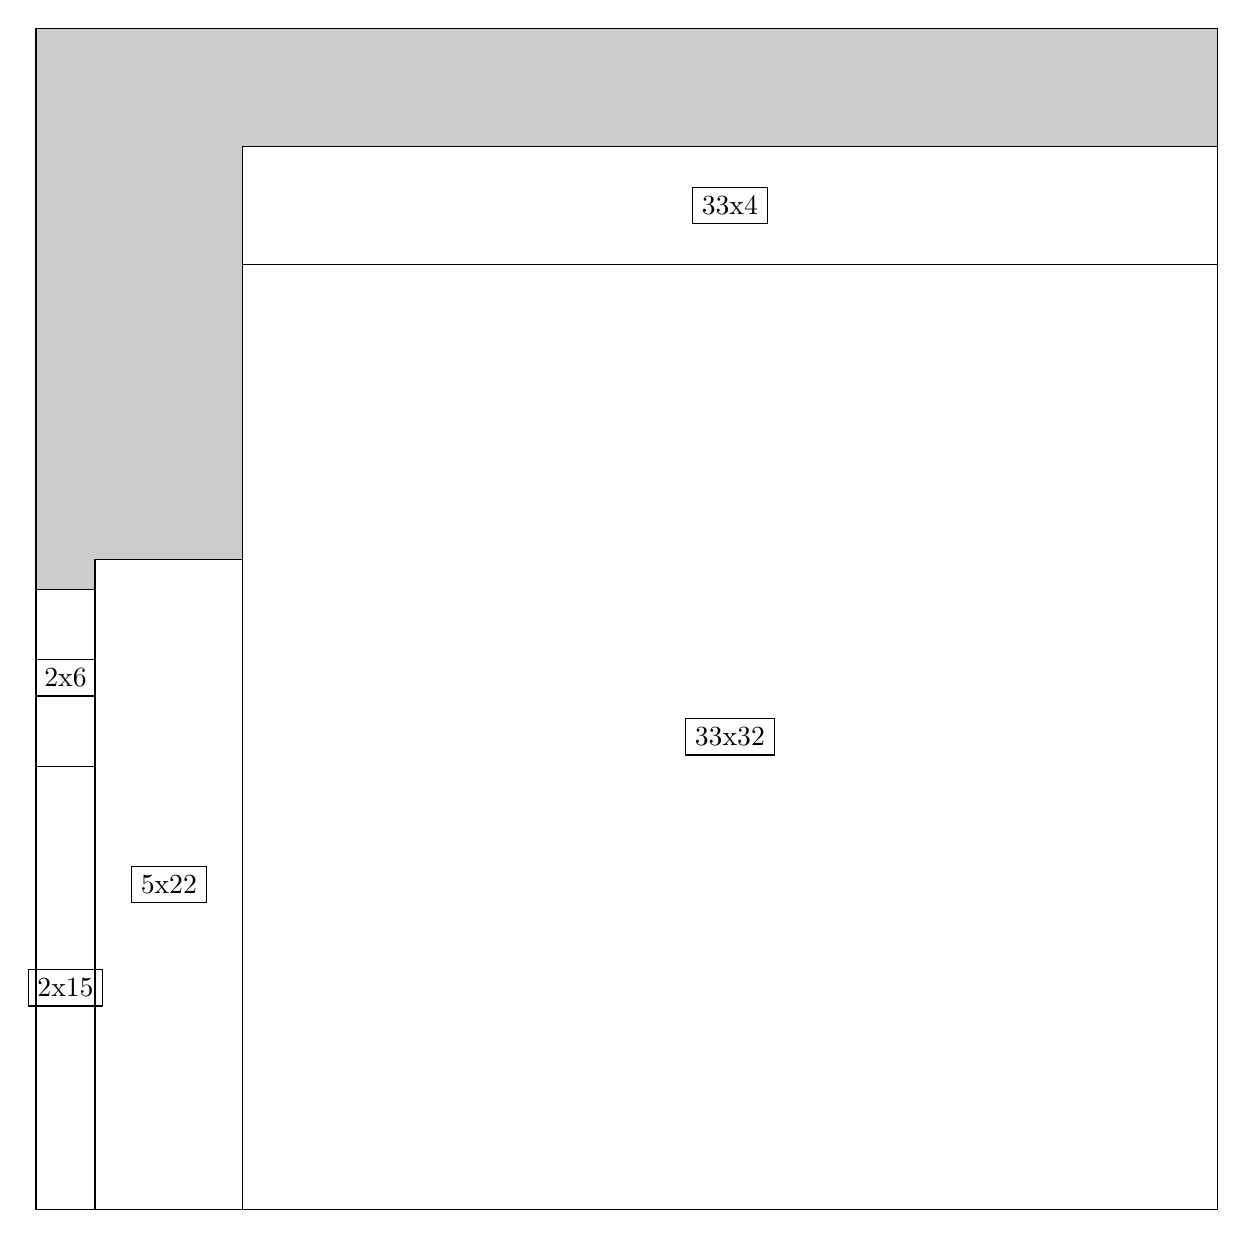
\begin{tikzpicture}[shorten >=1pt,scale=1.0,every node/.style={scale=1.0},->]
\tikzstyle{vertex}=[circle,fill=black!25,minimum size=14pt,inner sep=0pt]
\filldraw[fill=gray!40!white, draw=black] (0,0) rectangle (15.0,15.0);
\foreach \name/\x/\y/\w/\h in {33x32/2.625/0.0/12.375/12.0,33x4/2.625/12.0/12.375/1.5,5x22/0.75/0.0/1.875/8.25,2x15/0.0/0.0/0.75/5.625,2x6/0.0/5.625/0.75/2.25}
\filldraw[fill=white!40!white, draw=black] (\x,\y) rectangle node[draw] (\name) {\name} ++(\w,\h);
\end{tikzpicture}


w =33 , h =32 , x =7 , y =0 , v =1056
\par
w =33 , h =4 , x =7 , y =32 , v =132
\par
w =5 , h =22 , x =2 , y =0 , v =110
\par
w =2 , h =15 , x =0 , y =0 , v =30
\par
w =2 , h =6 , x =0 , y =15 , v =12
\par
\newpage


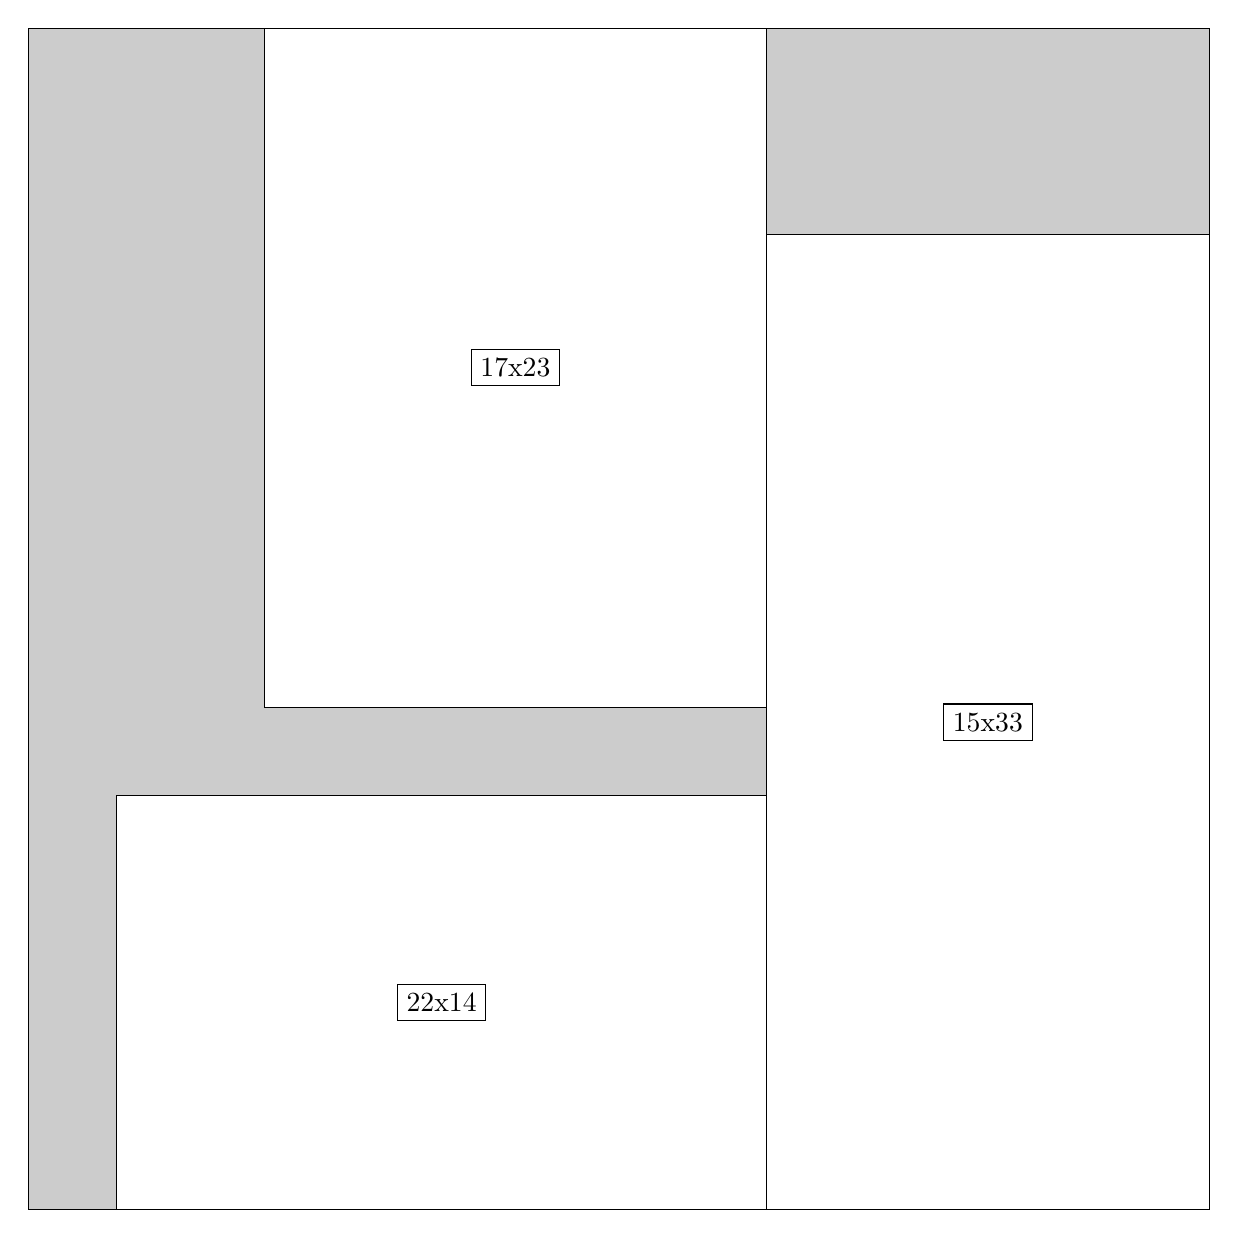
\begin{tikzpicture}[shorten >=1pt,scale=1.0,every node/.style={scale=1.0},->]
\tikzstyle{vertex}=[circle,fill=black!25,minimum size=14pt,inner sep=0pt]
\filldraw[fill=gray!40!white, draw=black] (0,0) rectangle (15.0,15.0);
\foreach \name/\x/\y/\w/\h in {15x33/9.375/0.0/5.625/12.375,22x14/1.125/0.0/8.25/5.25,17x23/3.0/6.375/6.375/8.625}
\filldraw[fill=white!40!white, draw=black] (\x,\y) rectangle node[draw] (\name) {\name} ++(\w,\h);
\end{tikzpicture}


w =15 , h =33 , x =25 , y =0 , v =495
\par
w =22 , h =14 , x =3 , y =0 , v =308
\par
w =17 , h =23 , x =8 , y =17 , v =391
\par
\newpage


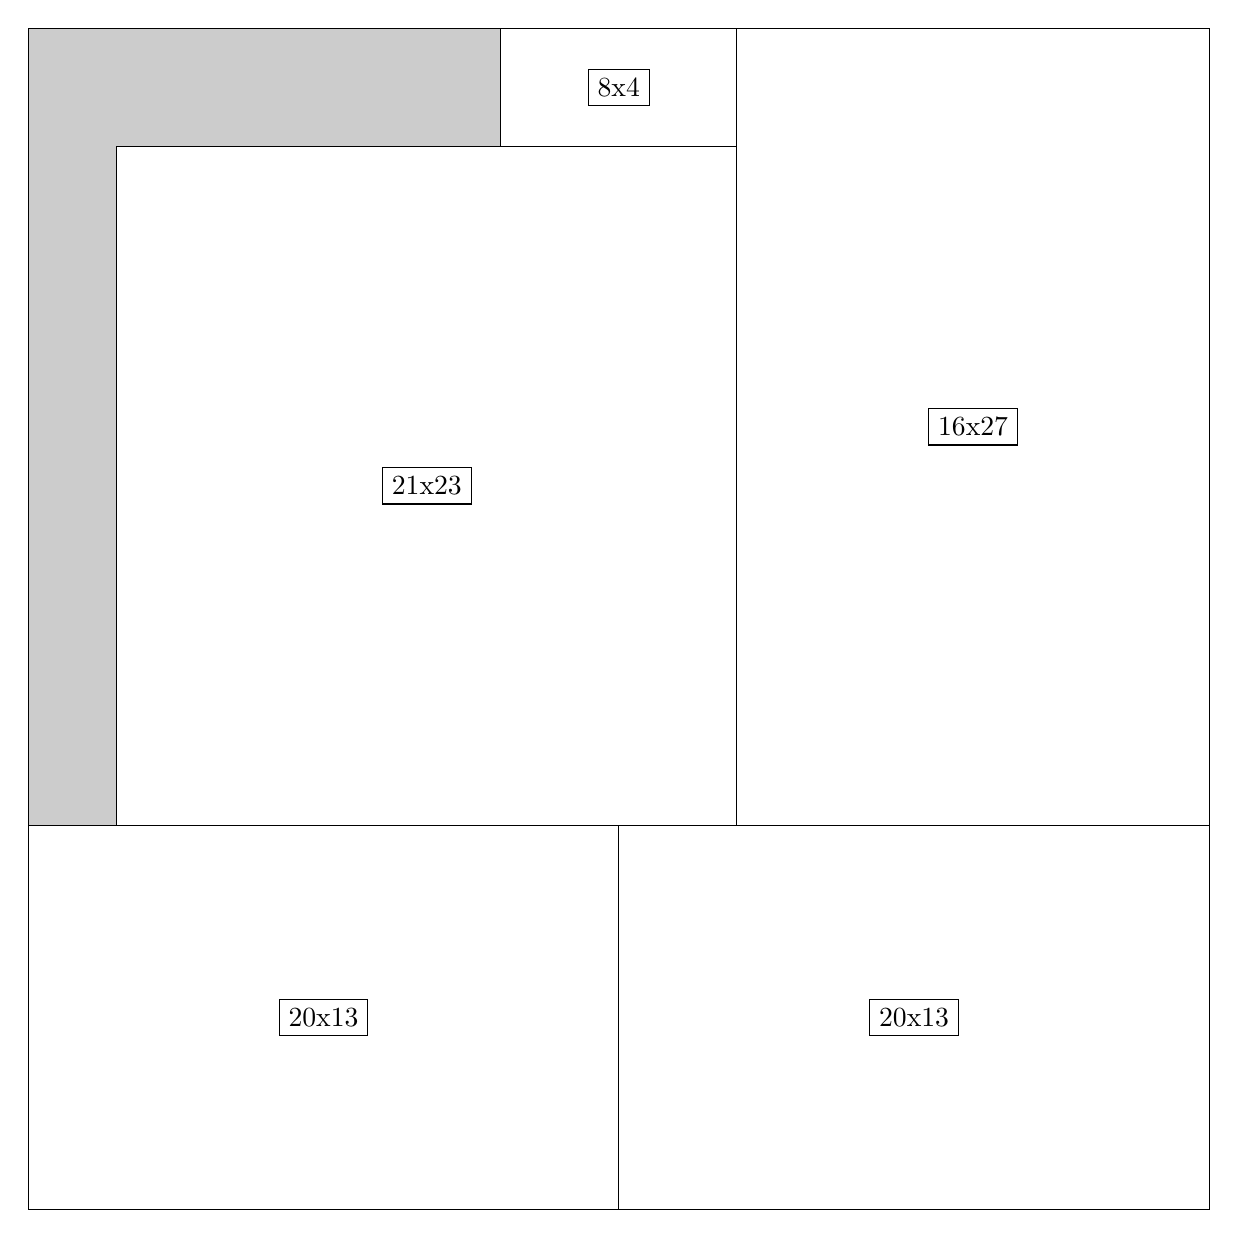
\begin{tikzpicture}[shorten >=1pt,scale=1.0,every node/.style={scale=1.0},->]
\tikzstyle{vertex}=[circle,fill=black!25,minimum size=14pt,inner sep=0pt]
\filldraw[fill=gray!40!white, draw=black] (0,0) rectangle (15.0,15.0);
\foreach \name/\x/\y/\w/\h in {20x13/7.5/0.0/7.5/4.875,20x13/0.0/0.0/7.5/4.875,16x27/9.0/4.875/6.0/10.125,21x23/1.125/4.875/7.875/8.625,8x4/6.0/13.5/3.0/1.5}
\filldraw[fill=white!40!white, draw=black] (\x,\y) rectangle node[draw] (\name) {\name} ++(\w,\h);
\end{tikzpicture}


w =20 , h =13 , x =20 , y =0 , v =260
\par
w =20 , h =13 , x =0 , y =0 , v =260
\par
w =16 , h =27 , x =24 , y =13 , v =432
\par
w =21 , h =23 , x =3 , y =13 , v =483
\par
w =8 , h =4 , x =16 , y =36 , v =32
\par
\newpage


\end{document}